\documentclass[11pt,a4paper]{article}

% -------------------- Packages --------------------
\usepackage[a4paper,margin=2.5cm]{geometry}
\usepackage{graphicx}
\usepackage{float}
\usepackage{booktabs}
\usepackage{amsmath}
\usepackage{siunitx}
\usepackage{hyperref}
\usepackage{xurl}
\usepackage{enumitem}
\usepackage{longtable}
\usepackage{caption}
\usepackage{subcaption}
\usepackage{cite}
\usepackage{tikz}
\usepackage{fancyhdr}
\setlength{\columnsep}{20pt}
\setlength{\voffset}{0.7cm}
\setlength{\headsep}{40pt}
\setlength{\headheight}{40pt}
\newcolumntype{L}[1]{>{\raggedright\arraybackslash}p{#1}}

% -------------------- Title Info --------------------
% Title page
\title{\textbf{Final Project}}
\author{Bujin Shao | bujin.shao@estudiantat.upc.edu\\Hemeng Wang | hemeng.wang@estudiantat.upc.edu\\Nai-Chi Cheng | nai-chi.cheng@estudiantat.upc.edu \\Saúl Daniel Castañeda Arzaga | saul.daniel.castaneda@estudiantat.upc.edu\\}
\date{\today}

% Header and footer
\pagestyle{fancy}
\fancyhead{}
\fancyhead[L]{\textbf{Control and Automation \\ for the Efficient Use of Energy}\\\textbf{CAPUEE 25-26}}
\fancyhead[R]{\textbf{Bujin Shao, Hemeng Wang\\Nai-Chi Cheng\\Saúl Daniel Castañeda Arzaga}}
\fancyfoot{}
\begin{document}
\maketitle

% ==================================================
\begin{abstract}
% Concise summary: problem, approach, prototype, results, key takeaway.
This project presents a smart hair dryer safety and energy management system that integrates real-time sensing, software-based control logic, and user-oriented feedback to address the limitations of conventional household hair dryers. Traditional devices operate in an open-loop manner with fixed thermal protection, applying uniform heat regardless of user-specific factors such as hair thickness, porosity, or environmental conditions, leading to potential energy waste and thermal damage.

The proposed system employs an ESP32 microcontroller connected to non-invasive current and temperature sensors (SCT013 and LM35) to continuously monitor operational parameters. A Python-based supervisory control system evaluates sensor data against dynamically generated safety protocols that incorporate hair characteristics and environmental factors obtained from external APIs. When unsafe conditions are detected—such as prolonged high-temperature exposure or excessive high-heat mode usage—the system automatically disconnects power via a relay module.

The prototype was validated through iterative hardware calibration and software testing, including simulation mode for hardware-independent verification. Key achievements include accurate RMS current measurement synchronized to AC frequency, duration-based threshold enforcement with hysteresis to prevent false alarms, and a user-friendly interface providing personalized drying recommendations and energy cost analysis. The system successfully demonstrates improved safety monitoring and energy efficiency awareness while maintaining practical usability for household hair care applications.
\end{abstract}
\newpage
\tableofcontents

% ==================================================
\newpage
\section{Introduction}

\subsection{Background \& Motivation}

Energy efficiency and safety in household appliances have become increasingly important in the context of rising electricity costs, environmental sustainability goals, and consumer awareness of product safety. Hair dryers, as one of the most power-intensive portable household devices, typically operate at 1,200--1,800 watts and are used regularly by millions of people worldwide. Despite their widespread use and significant energy consumption, conventional hair dryers lack adaptive control mechanisms that account for user-specific needs or environmental conditions.

From a safety perspective, excessive heat exposure poses a documented risk of hair damage through protein denaturation, moisture loss, and structural weakening of hair fibers. Different hair types exhibit vastly different thermal sensitivities: fine hair with high porosity requires gentle heat application, while thick hair with low porosity may tolerate higher temperatures for effective drying. However, standard devices provide no guidance or automatic adjustment based on these factors, placing the burden entirely on the user to manually regulate heat and duration.

From an energy efficiency perspective, users often lack real-time feedback on power consumption or cost, leading to suboptimal usage patterns. Additionally, environmental factors such as ambient temperature and humidity significantly affect natural drying rates, yet these are rarely considered when selecting blow-drying settings. The absence of intelligent control results in both wasted energy and increased thermal stress on hair.

Furthermore, dynamic electricity pricing structures increasingly incentivize off-peak usage and efficient consumption patterns. A smart hair dryer system that integrates real-time pricing data and environmental sensing could provide users with actionable recommendations to reduce both energy costs and thermal damage while maintaining convenience.

This project addresses these challenges by developing a prototype control and automation system for efficient and safe hair dryer operation, combining embedded sensing, supervisory control software, and external data integration to demonstrate the feasibility of intelligent, user-aware household appliances.

\subsection{Project Goals}

The primary objective of this project is to design, implement, and validate a smart hair dryer control system that enhances both operational safety and energy efficiency through real-time monitoring and adaptive decision-making. Specific goals include:

\begin{enumerate}
  \item \textbf{Real-time Sensing and Measurement:} Implement accurate current and temperature sensing using non-invasive sensors interfaced with an ESP32 microcontroller, achieving stable measurements suitable for safety-critical decision-making.

  \item \textbf{Dynamic Safety Protocol Generation:} Develop a protocol calculator that adapts safety thresholds and recommended usage patterns based on user-specific parameters (hair type, hair porosity) and environmental conditions (ambient temperature, humidity).

  \item \textbf{Automated Safety Enforcement:} Design and implement a supervisory control system capable of detecting unsafe operating conditions and automatically disconnecting power through a relay module when safety limits are exceeded, with hysteresis to prevent false alarms.

  \item \textbf{User-Oriented Feedback and Recommendations:} Create an interface that provides users with personalized drying protocols, including recommended heat settings, phase durations, and estimated energy costs based on real-time electricity pricing.

  \item \textbf{System Robustness and Testability:} Ensure the system operates reliably in both hardware-connected and simulation modes, with graceful degradation when external APIs are unavailable, enabling comprehensive testing and validation.

  \item \textbf{Practical Validation:} Validate the prototype through iterative calibration and testing using a real household hair dryer (Xiaomi 1,600 W model) to demonstrate feasibility in realistic operating conditions.
\end{enumerate}

Success is measured by the system's ability to consistently detect and respond to unsafe conditions, provide stable and accurate sensor readings, operate in both hardware and simulation modes, and deliver interpretable feedback that empowers users to make informed decisions regarding energy efficiency and hair care safety.

\subsection{Overview of the Proposed Solution}
% High-level principle: sense (current + temperature) -> decide -> actuate + recommend schedule via price API
\begin{figure}[H]
  \centering
    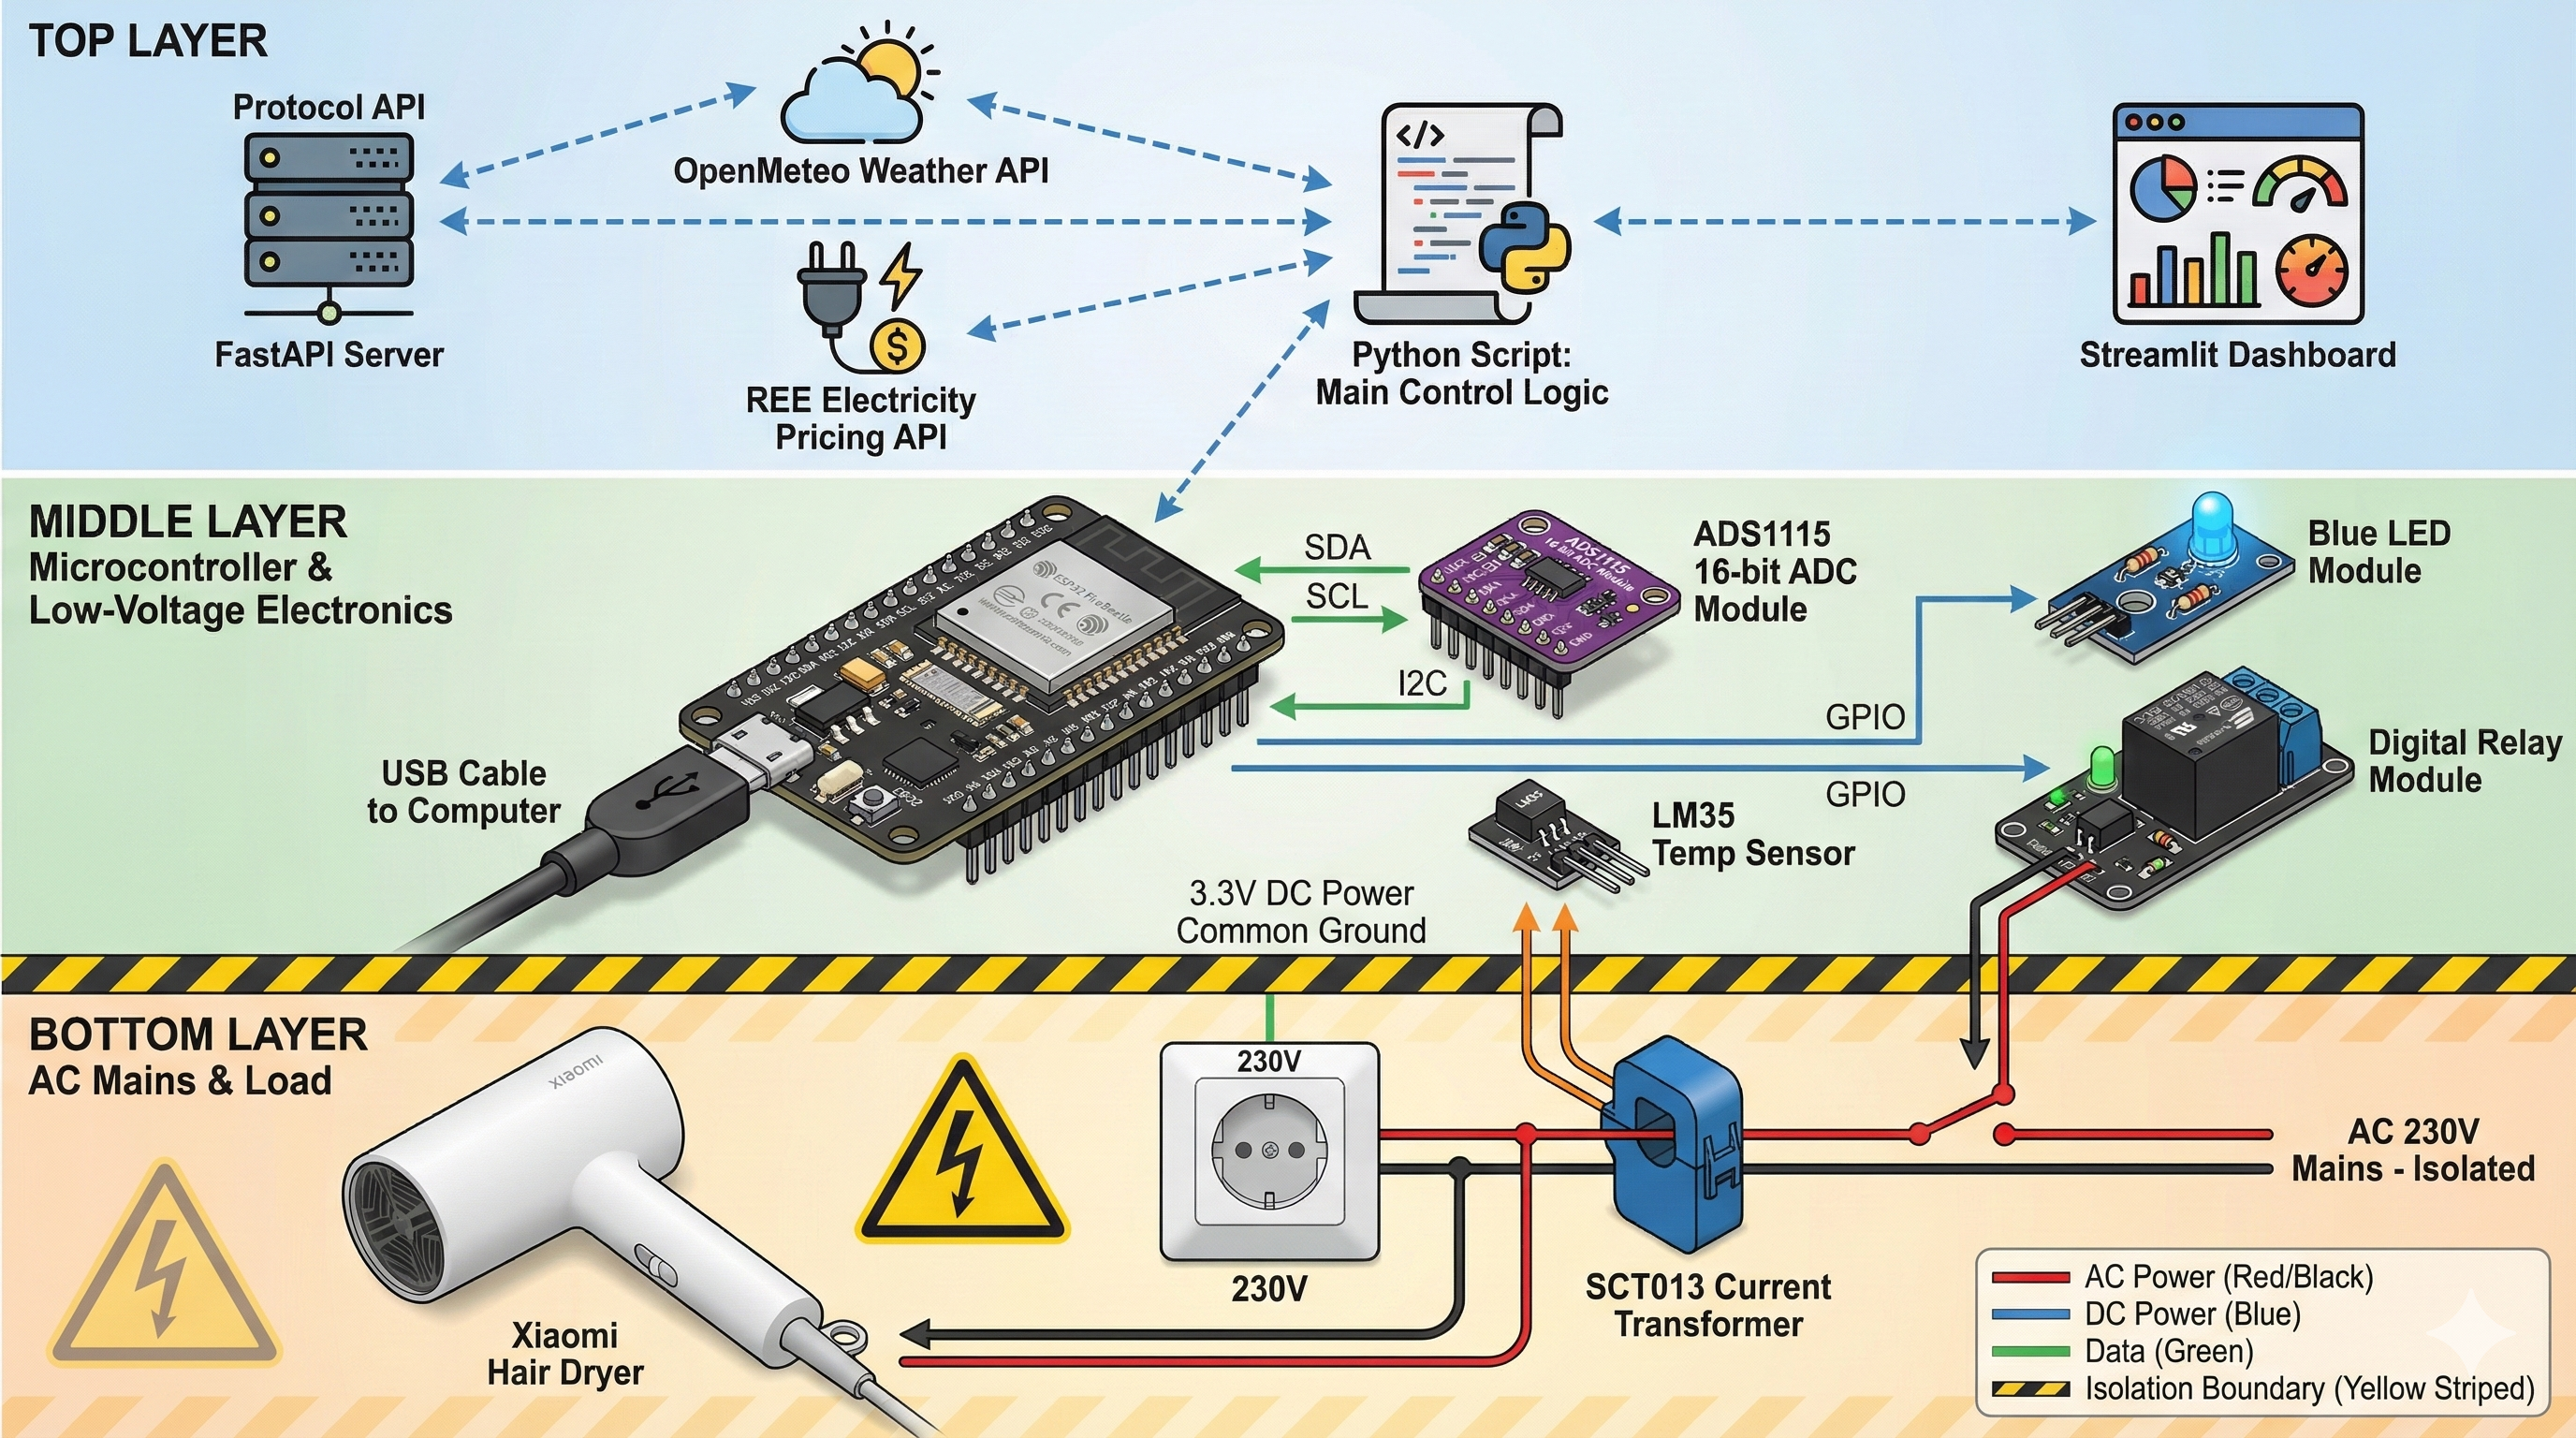
\includegraphics[width=1\linewidth]{figures/System schematic of the prototype.png}
   
   \caption{System schematic of the prototype.}
  \label{fig:system-flow}
\end{figure}

The diagram illustrates a three-layer architecture. The \textcolor{red}{bottom layer (red)} handles high-voltage AC mains (230V) with the Xiaomi hair dryer load, SCT013 current transformer clamped on the live conductor for non-invasive sensing, and a digital relay (HF3FA) for automated power cutoff, all isolated from low-voltage electronics. The \textcolor{blue}{middle layer (blue)} comprises low-voltage (3.3V DC) electronics including the FireBeetle ESP32 microcontroller, ADS1115 16-bit ADC for current signal digitization (with bias and conditioning), LM35 temperature sensor near the air outlet, blue LED for status feedback, and USB/serial connection to the host computer running Python control logic. The \textcolor{green}{top layer (green)} features external APIs (FastAPI for dynamic hair-dry protocols incorporating hair type/porosity and environment; Open-Meteo for weather; REE for pricing), Python script for supervisory safety strategy (threshold enforcement with hysteresis), and Streamlit dashboard for user recommendations/energy visualization.

\newpage

\subsection{Overview of Control}

An existing hair drying protocol \cite{lee_hair_damage} is used to determine a dynamic control strategy based on user-specific hair properties (e.g., hair thickness and porosity), environmental conditions (temperature and relative humidity retrieved via Open-Meteo), and user preferences (e.g., towel-dry level and time-priority).
These inputs are processed in \texttt{protocol\_calculator.py} to generate (i) personalized drying recommendations (heat level and phase durations) and (ii) a machine-enforceable safety protocol consisting of temperature/current thresholds and associated maximum allowable durations.

\paragraph{Protocol generation (recommended schedule and limits).}
The protocol calculation computes a \emph{drying power index} (DP) from ambient temperature and humidity to represent how much the environment contributes to moisture removal; DP then adjusts the recommended blow-drying time and heat aggressiveness. Using DP together with hair thickness/porosity and time-priority, the algorithm selects a discrete heat setting (Low/Medium/High) and estimates a two-stage schedule: a main (bulk) drying phase and a styling/finish phase, optionally recommending hybrid air-drying plus blow-drying in favorable conditions to reduce energy use and thermal stress.
Because excessive heat exposure and prolonged drying time are linked to structural hair shaft damage, the same computed phase durations are reused as time limits for safety enforcement. % \cite{lee_hair_damage}

\paragraph{Measured indicators of dryer ``mode''.}
In a typical consumer hair dryer, different user-selected modes (e.g., low vs.\ high heat) manifest as different electrical and thermal signatures.
The system therefore uses measured RMS current as a proxy for sustained high-heat usage, and outlet air temperature as a proxy for thermal exposure at the device boundary that is relevant to the user. 

\paragraph{Supervisory safety enforcement (runtime monitoring and actuation).}
The method of control employs a supervisory safety strategy in \texttt{safety\_strategy.py} that monitors real-time temperature and RMS current at the same cadence as the incoming sensor stream (every few seconds in the prototype implementation).
For each constraint (temperature and current), the controller starts a violation timer when the measurement exceeds the protocol threshold; shutdown is triggered only if the violation persists continuously for the configured duration (e.g., total allowed drying time for temperature, and bulk-phase time for high-current/high-heat operation).
Hysteresis is implemented by resetting the corresponding timer whenever the measurement returns to a safe range, which reduces false trips from brief spikes during normal handling.
Finally, an absolute maximum runtime limit acts as a fail-safe (independent of protocol thresholds) to protect against abnormal usage or sensor/API failures; on shutdown, a relay is opened to disconnect power to the hair dryer.

\paragraph{In a representative use case:} for medium-thickness hair, normal porosity, 80\% towel-dried in Barcelona (18\textdegree C, 55\% humidity, DP=0.43), the protocol recommends low-heat bulk phase (3.2 min at 800W, 64 Wh) followed by styling (1.0 min at 800W, 13.3 Wh), totaling 77 Wh (0.020 EUR at 0.26 EUR/kWh) versus 125 Wh (0.0325 EUR) for unguided high-heat usage (5 min at 1500W), achieving 36--48 Wh savings per session; sustained high-heat violation triggers ``You used too long the high heat mode in your hairdryer'', actuating relay cutoff.
% ==================================================

% ==================================================
\newpage
\section{Project Description \& Workflow}

\subsection{Problem Statement}
% What problem are you solving with the smart hair dryer?
Conventional household hair dryers operate largely in an open-loop fashion at the system level, with user-selected heat and airflow settings and only fixed, hardware-based thermal protection.

In addition, users exhibit significant variability in hair properties, such as hair thickness and hair porosity, which strongly influence heat absorption, moisture retention, and drying dynamics. However, conventional hair dryers apply identical thermal behavior regardless of these differences, potentially resulting in unnecessary energy consumption or increased thermal stress.

Furthermore, users lack intuitive information regarding electrical energy usage, thermal risk, and optimal drying strategies under varying environmental conditions, such as ambient temperature and humidity.

The problem addressed in this project is therefore the design of a smart hair dryer control system capable of monitoring real-time electrical current and temperature, adapting its behavior based on hair thickness and porosity, and enforcing safety constraints to improve both energy efficiency and operational safety.
\subsection{Overview of the Proposed Solution}
% High-level principle: sense (current + temperature) -> decide -> actuate + recommend schedule via price API
To address the identified challenges, this project proposes a smart hair dryer control system that integrates real-time sensing, software-based decision logic, and user-oriented feedback.

The system follows a high-level sense--decide--actuate paradigm. Electrical current and temperature are continuously measured using an embedded microcontroller. These measurements are transmitted to a supervisory control program, which evaluates them against safety rules and operational constraints dynamically generated by an external API.

The generated protocol incorporates user-specific parameters, including hair thickness and hair porosity, as well as environmental conditions such as ambient temperature and humidity. Based on this evaluation, the control system can automatically actuate a relay to disconnect the hair dryer when unsafe conditions are detected.

In parallel, the system provides recommended drying schedules and energy-related feedback to the user through a graphical interface, allowing users to better understand the relationship between hair properties, energy consumption, and safety behavior.

\subsection{System Flow / Workflow Diagram}
% Insert diagram: sensors -> ESP32 -> control logic -> actuators + data logging/UI + external API
\begin{figure}[H]
  \centering
  \begin{tikzpicture}[
    node distance=2cm and 2.5cm,
    box/.style={rectangle, draw, fill=blue!10, text width=2cm, align=center, rounded corners, minimum height=0.9cm, font=\small},
    sensor/.style={rectangle, draw, fill=orange!20, text width=2cm, align=center, rounded corners, minimum height=0.9cm, font=\small},
    logic/.style={rectangle, draw, fill=cyan!20, text width=1.9cm, align=center, rounded corners, minimum height=1cm, font=\small},
    actuator/.style={rectangle, draw, fill=yellow!20, text width=1.8cm, align=center, rounded corners, minimum height=0.9cm, font=\small},
    api/.style={rectangle, draw, fill=green!20, text width=2cm, align=center, rounded corners, minimum height=1cm, font=\small},
    arrow/.style={->, >=stealth, thick}
  ]

    \node[sensor] (sensor) at (0,-1.5) {Current \& Temp\\Sensor};
    \node[box, text width=1.7cm] (esp) at (3,-1.5) {ESP32\\Micro-\\controller};
    \node[logic] (logic) at (6,-1.5) {Supervisory\\Logic};

    \node[actuator] (relayled) at (3,0) {Relay \&\\LED};
    \node[actuator] (hairdryer) at (0,0) {Hairdryer};

    \node[api] (proto) at (9,-1.5) {Hairdry\\Protocol\\Generator};
    \node[api] (ui) at (9,0) {User\\Interface};
    \node[api] (api) at (6,0) {API\\Services};

    \draw[arrow] (hairdryer) to[out=180, in=180]node[left, font=\small] {(environment)} (sensor);
    \draw[arrow] (sensor) -- (esp);
    \draw[arrow] (esp) -- (logic);
    \draw[arrow] (logic) -- (esp);
    \draw[arrow] (logic) -- (relayled);
    \draw[arrow] (relayled) -- (hairdryer);
    \draw[arrow] (logic) -- (proto);
    \draw[arrow] (proto) -- (logic);
    \draw[arrow] (proto) -- (ui);
    \draw[arrow] (ui) -- (proto);
    \draw[arrow] (api) -- (proto);
    \vspace{1em}
  \end{tikzpicture}
  \vspace{.5em}
  \caption{System workflow.}
  \label{fig:workflow}
\end{figure}

Sensor measurements are acquired by the ESP32 microcontroller and forwarded to a Python-based supervisory control logic for real-time evaluation.

The supervisory control logic acts as the central decision unit, comparing sensor data with dynamically generated safety protocols obtained from an external API. Based on this evaluation, control commands are issued to the relay and LED module to actuate the hair dryer.

The color coding highlights different system layers: blue blocks represent sensing and control logic, while yellow blocks denote the physical actuation layer and green
blocks represnet a separate user interface visualizes system status and recommendations without directly affecting hardware control.
% Optional but often helpful:
\subsection{Requirements \& Success Criteria}
% Define what “works” means: sampling rate, RMS stability, temp thresholds, relay/LED behavior, API refresh cadence
% ==================================================


\paragraph{Functional Requirements}
The system shall:
\begin{itemize}
  \item Measure electrical current and temperature in real time during hair dryer operation.
  \item Compute stable RMS current values suitable for safety monitoring.
  \item Adapt safety thresholds based on hair thickness and hair porosity.
  \item Automatically disconnect the hair dryer via a relay when predefined safety limits are exceeded.
  \item Retrieve and apply safety protocols dynamically from an external API.
  \item Provide real-time visualization of system status and energy-related information.
\end{itemize}


\paragraph{Success Criteria}
The project is considered successful if:
\begin{itemize}
  \item Unsafe operating conditions consistently result in timely disconnection of the hair dryer.
  \item Sensor measurements are stable and correctly reflected in both the control logic and user interface.
  \item The system operates reliably in both hardware-in-the-loop and simulation modes.
  \item Users receive clear and interpretable feedback regarding energy usage and safety behavior.
\end{itemize}

\newpage
\section{Prototype Development --- Hardware}

\subsection{Load of Choice}
% Hair dryer: rated power, modes, expected current range, safety considerations, measurement approach

\noindent The \emph{Xiaomi High-speed Ionic Hair Dryer} Model GSHGL01LX is used as the primary electrical load. With a rated power of 1600 W at a mains voltage of 220–240 V, it is suitable for validating our sensing and control system in a household context. It is also commonplace, as one of the team members already owned the unit, simplifying setup and data collection. Specifics: \begin{itemize}
    \item A high-speed internal motor is used for efficient airflow and drying, reflecting typical household power consumption patterns of motorized heaters.
    \item The nominal electrical characteristics—220–240 V~ at up to 1600 W—yield a current draw of approximately 7 A at rated conditions, which is a useful range for testing the robustness of our current transformer and ADC interface.
    \item Using a real shunt load like a hair dryer adds practical relevance to the project compared to purely resistive or artificial loads, and allows us to observe non-idealities such as inrush currents and thermal effects that occur during typical usage.
    \item The device includes a detachable nozzle, making it a relevant choice for evaluating non-invasive current sensing and thermal monitoring for the prototype by inserting the sensors between the nozzle and the main outlet.
\end{itemize}

\begin{table}[H]
  \hfill
  \centering
  \begin{minipage}[t]{0.7\textwidth}
    \centering
    \caption{Specifications of the Hair Dryer (Xiaomi GSHGL01LX)~\cite{xiaomi_hairdryer_specs}.}
    \label{tab:hairdryer_specs}
    \begin{tabular}{ll}
      \toprule
      Attribute & Value \\
      \midrule
      Model & GSHGL01LX \\
      Rated Voltage & 220--240 V~ \\ 
      Rated Frequency & 50--60 Hz \\ 
      Rated Power & 1600 W \\ 
      Product Dimensions & 128.6 × 70 × 231 mm (without nozzle) \\ 
      Power Cord Length & 1.7 m \\ 
      Net Weight & 406 g (without nozzle and cord) \\
      \bottomrule
    \end{tabular}
  \end{minipage}%
  \hfill
  \begin{minipage}[t]{0.2\textwidth}
    \centering
    \captionof{figure}{Actual product.}
    \label{fig:hairdryer_image}
    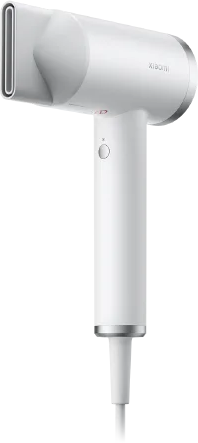
\includegraphics[width=0.6\linewidth]{figures/Xiaomi High-speed Ionic Hair Dryer.png}
  \end{minipage}
  \hfill
  \vspace{1em}
\end{table}


\subsection{Electronics}


\noindent Figure~\ref{fig:hardware_schematic} on the next page shows a schematic of the electronics of the prototype. The design integrates the mains-powered hairdryer with low-voltage sensing and control electronics, while maintaining isolation between high-voltage and low-voltage domains.

\paragraph{}Specifically, the hair dryer is connected to the AC mains, passing through an analog current transformer (SCT013) for real-time, non-invasive current measurement. The sensor output is conditioned, then digitized using an analog-to-digital converter (ADS1115), which communicates with a microcontroller (FireBeetle ESP32) via an I\textsuperscript{2}C bus. A temperature sensor module (LM35) is placed near the air outlet of the hair dryer, also connected to the microcontroller. A computer (not shown) handles control logic during testing to avoid reprogramming the microcontroller, which manages sensing and actuating. Control logic is not integrated for this prototype. All low-voltage components are powered from regulated DC supplies and share a common ground, while the AC side remains physically and electrically isolated for safety.


\begin{figure}[H]
  \centering
  
\includegraphics[width=.6\linewidth]{figures/ACEE_HardwareSchematic.pdf}
  \caption{Hardware schematic of the prototype.}
  \label{fig:hardware_schematic}
\end{figure}


% Table of parts: ESP32 FireBeetle, SCT013, ADS1115, DS18B20, relay/LED, resistors, wiring, enclosure, etc.
\begin{table}[H]
  \centering
  \begin{tabular}{lll}
    \toprule
    Component & Model & Purpose \\
    \midrule
    Microcontroller & ESP32 FireBeetle & Control + connectivity \\
    I/O expansion shield & Gravity & Wiring simplification \\
    ADC module (16-bit) & ADS1115 & High-resolution sampling \\
    Current sensor & SCT013 & Non-invasive AC current sensing \\
    Temperature sensor module & LM35 (DFR0023) & Outlet air temperature \\
    Digital relay module & HF3FA (DFR0473) &  Actuator: power cutoff \\
    LED module & DFR0021-B & Actuator: user feedback \\
    
    \bottomrule
  \end{tabular}
  \caption{Bill of materials.}
\end{table}

\begin{figure}[H]
\centering    
    % Row 1
    \begin{subfigure}[t]{0.3\textwidth}
        \centering
        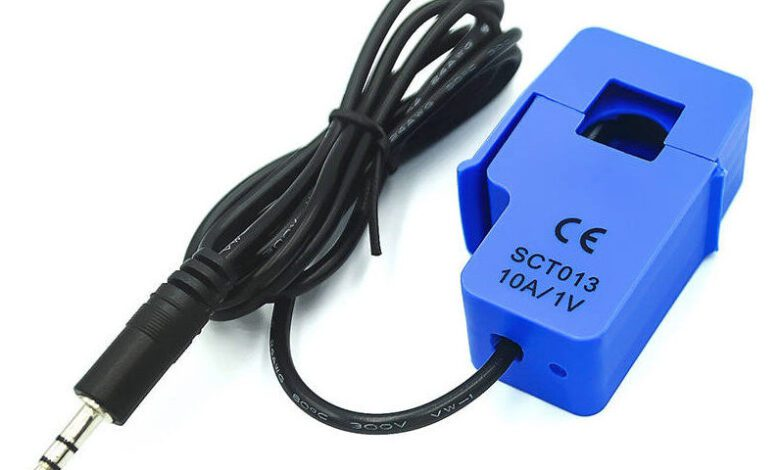
\includegraphics[height=2.4cm, keepaspectratio]{figures/SCT013_CurrentSensor.jpeg}
        \caption{SCT013 Current Sensor~\cite{yhdc_sct013}}
        \label{fig:SCT013}
    \end{subfigure}
    \hfill
    \begin{subfigure}[t]{0.3\textwidth}
        \centering
        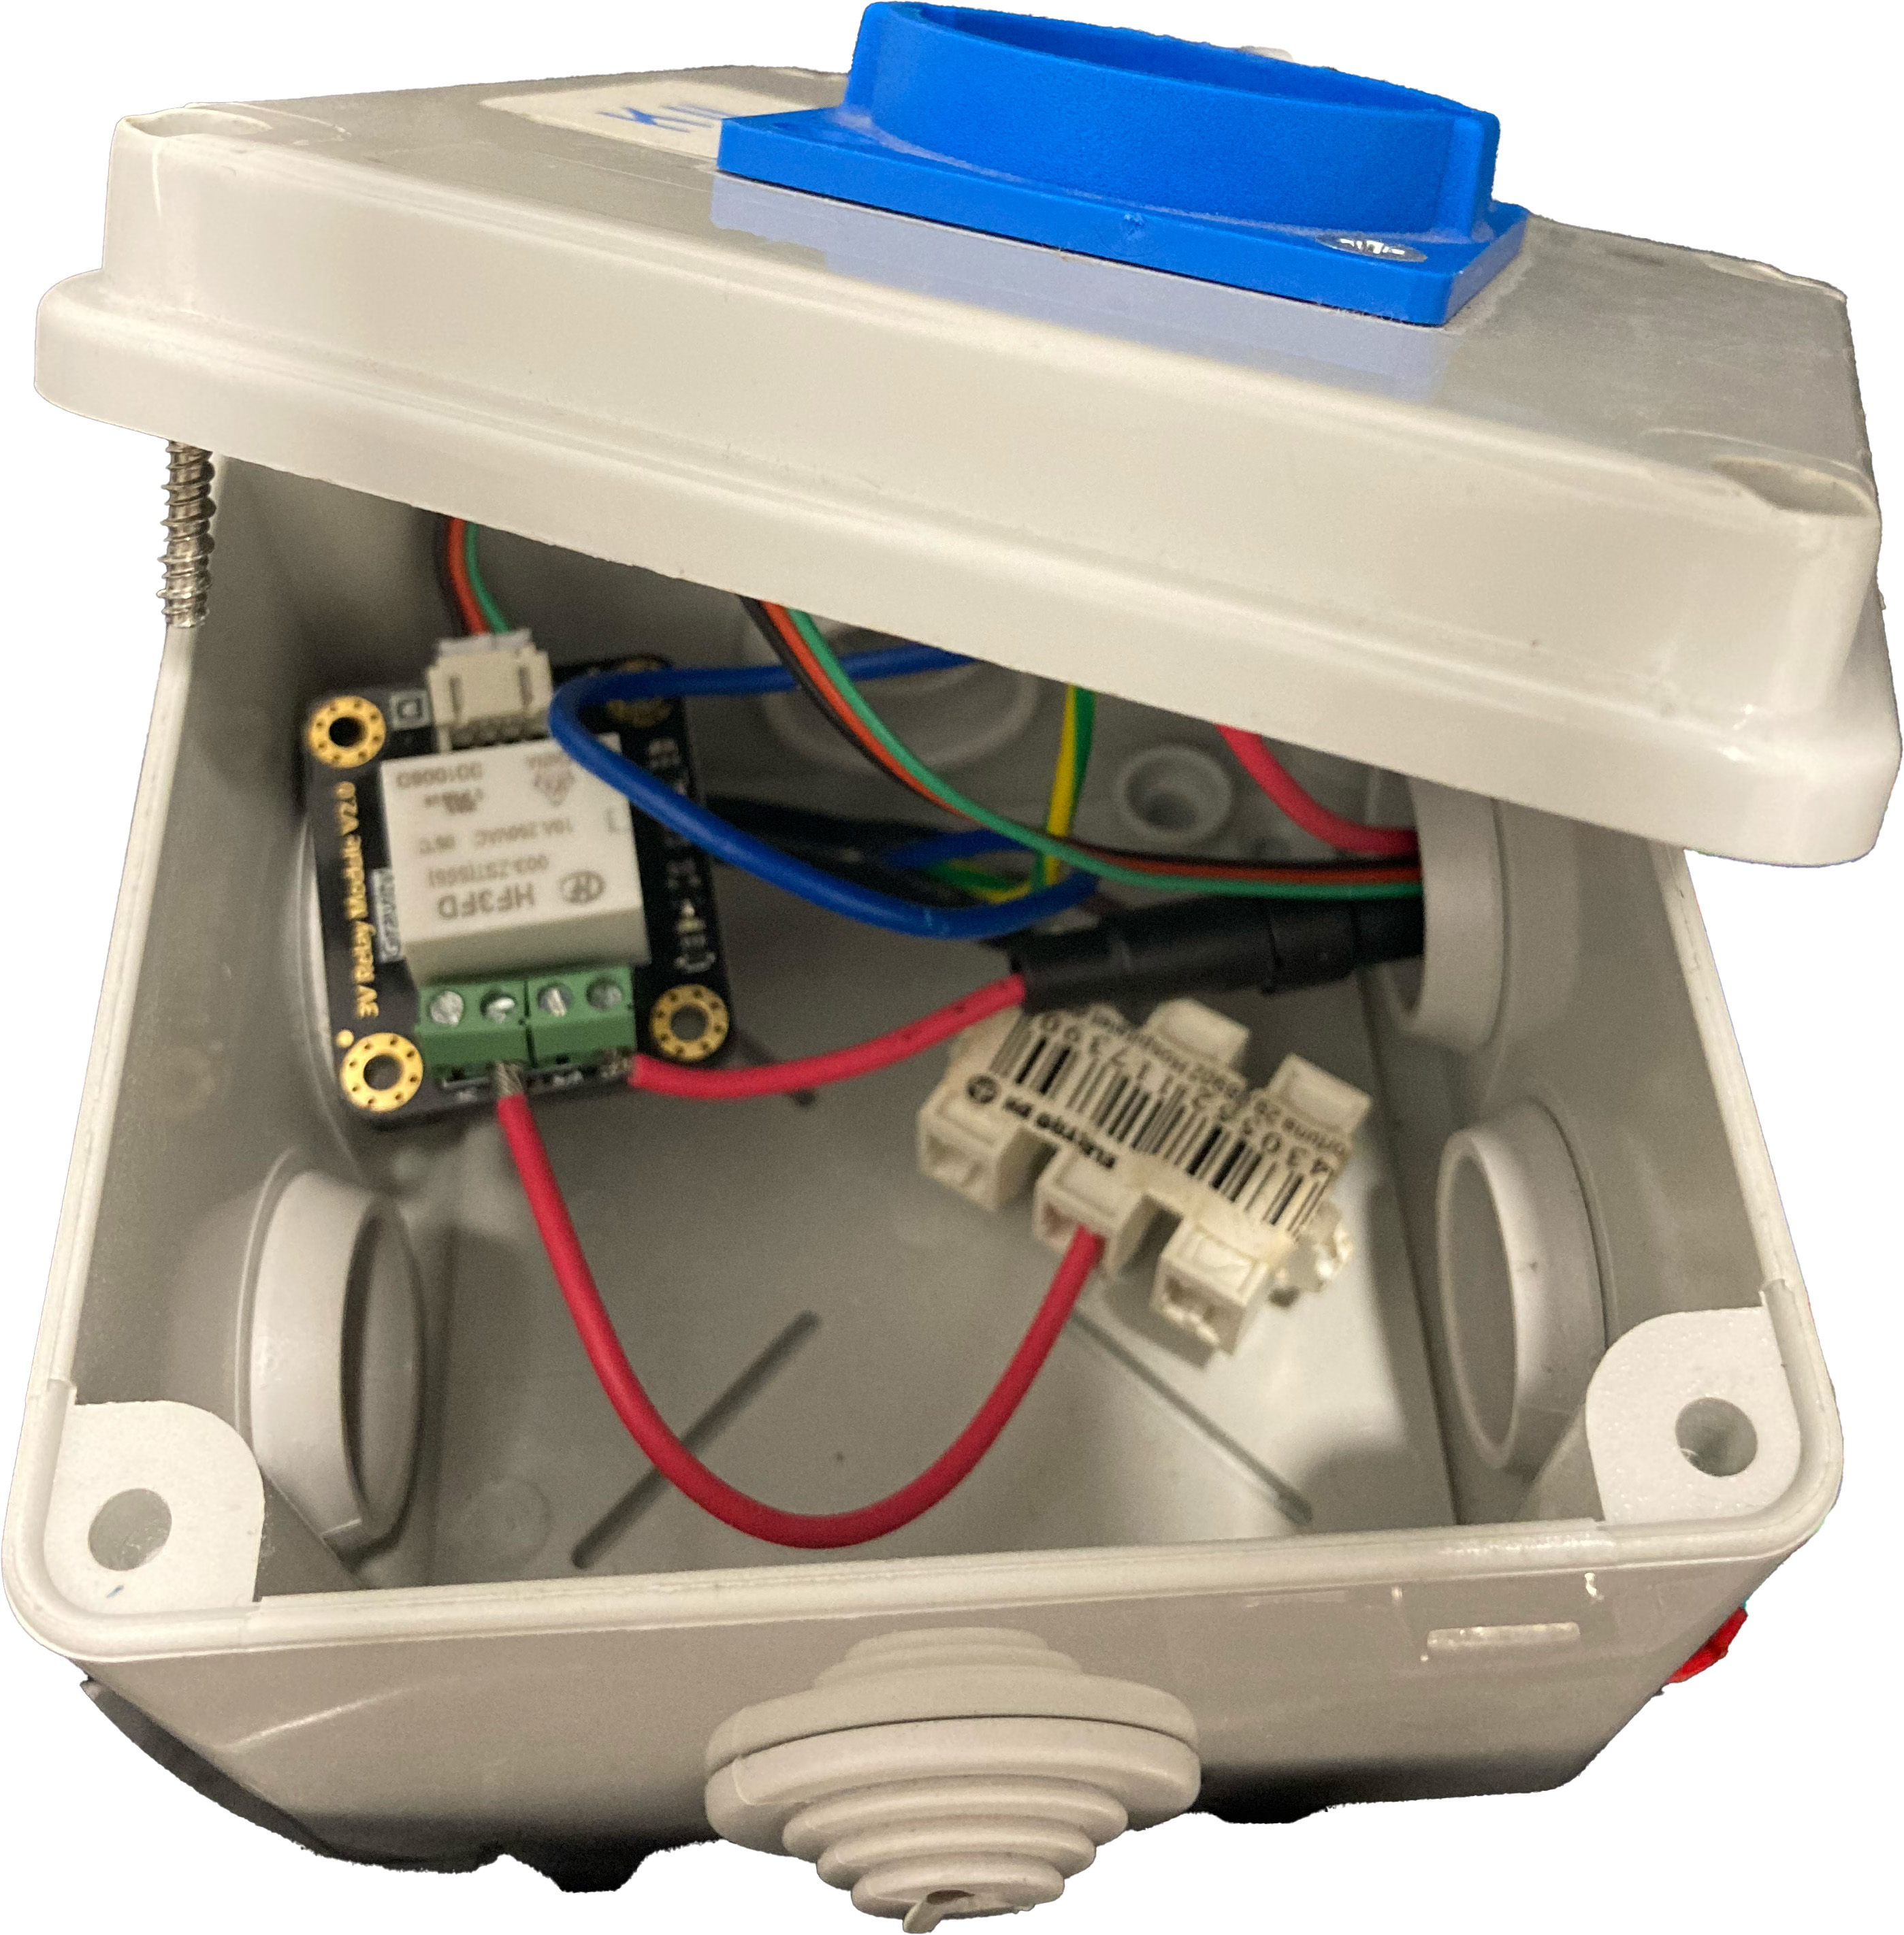
\includegraphics[height=2.4cm, keepaspectratio]{figures/ABB_SocketBox.jpg}
        \caption{Socket box with fuse and the relay in (c)}
        \label{fig:SocketBox}
    \end{subfigure}
    \hfill
    \begin{subfigure}[t]{0.3\textwidth}
        \centering
        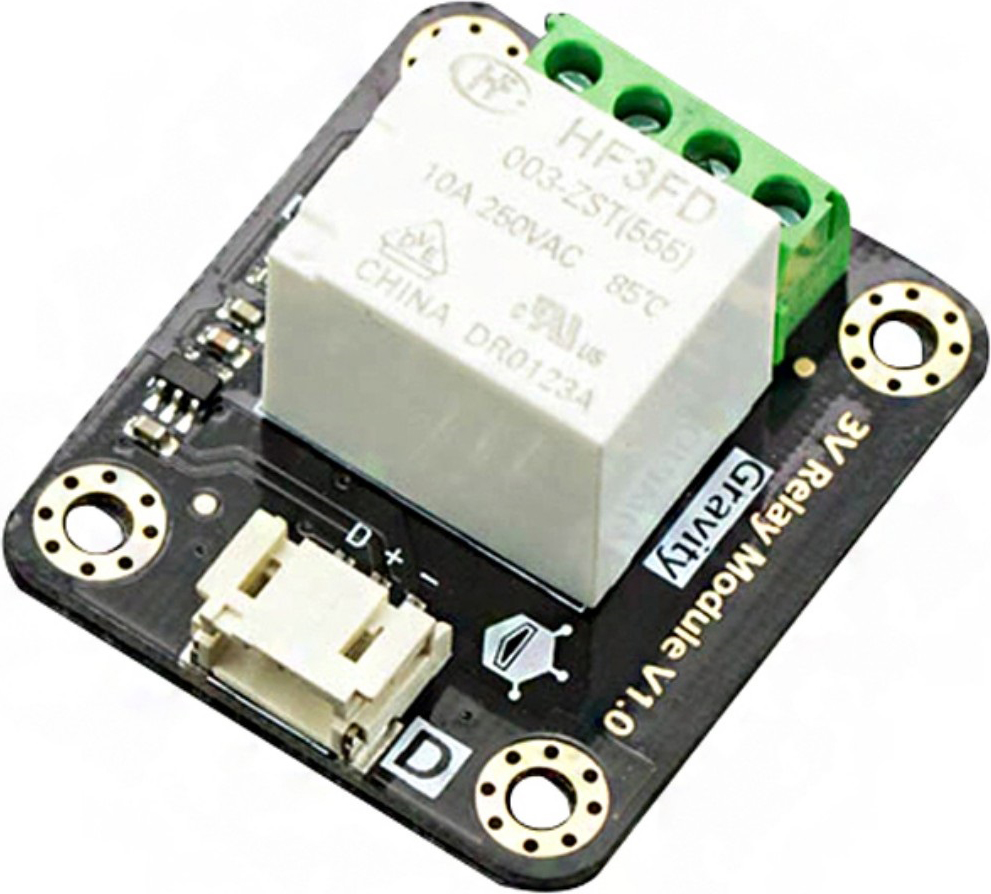
\includegraphics[height=2.4cm, keepaspectratio]{figures/GravityDigital10A_Relay.jpg}
        \caption{HF3FA Relay~\cite{dfrobot_relay_module_dfr0473}}
        \label{fig:HF3FD}
    \end{subfigure}
    
    % Row 2
    \begin{subfigure}[t]{0.3\textwidth}
        \centering
        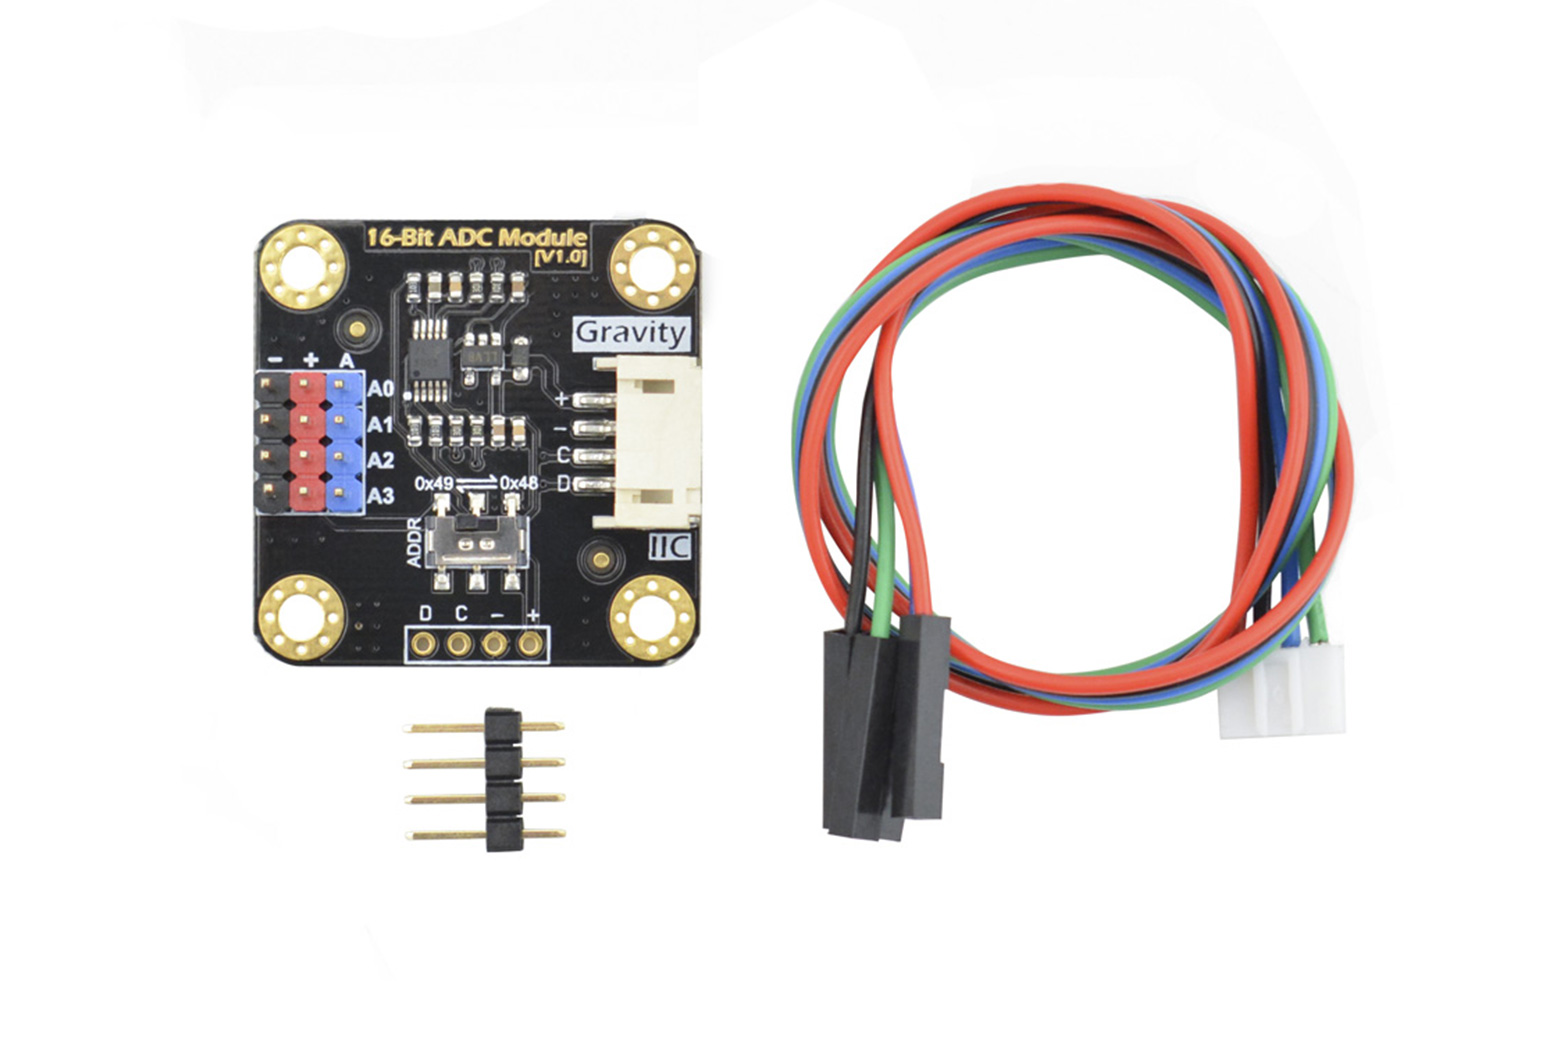
\includegraphics[height=2.4cm, keepaspectratio]{figures/ADS1115_16bitADCModule.jpg}
        \caption{ADS1115 ADC~\cite{ti_ads1115}}
        \label{fig:ADS1115}
    \end{subfigure}
    \hfill
    \begin{subfigure}[t]{0.3\textwidth}
        \centering
        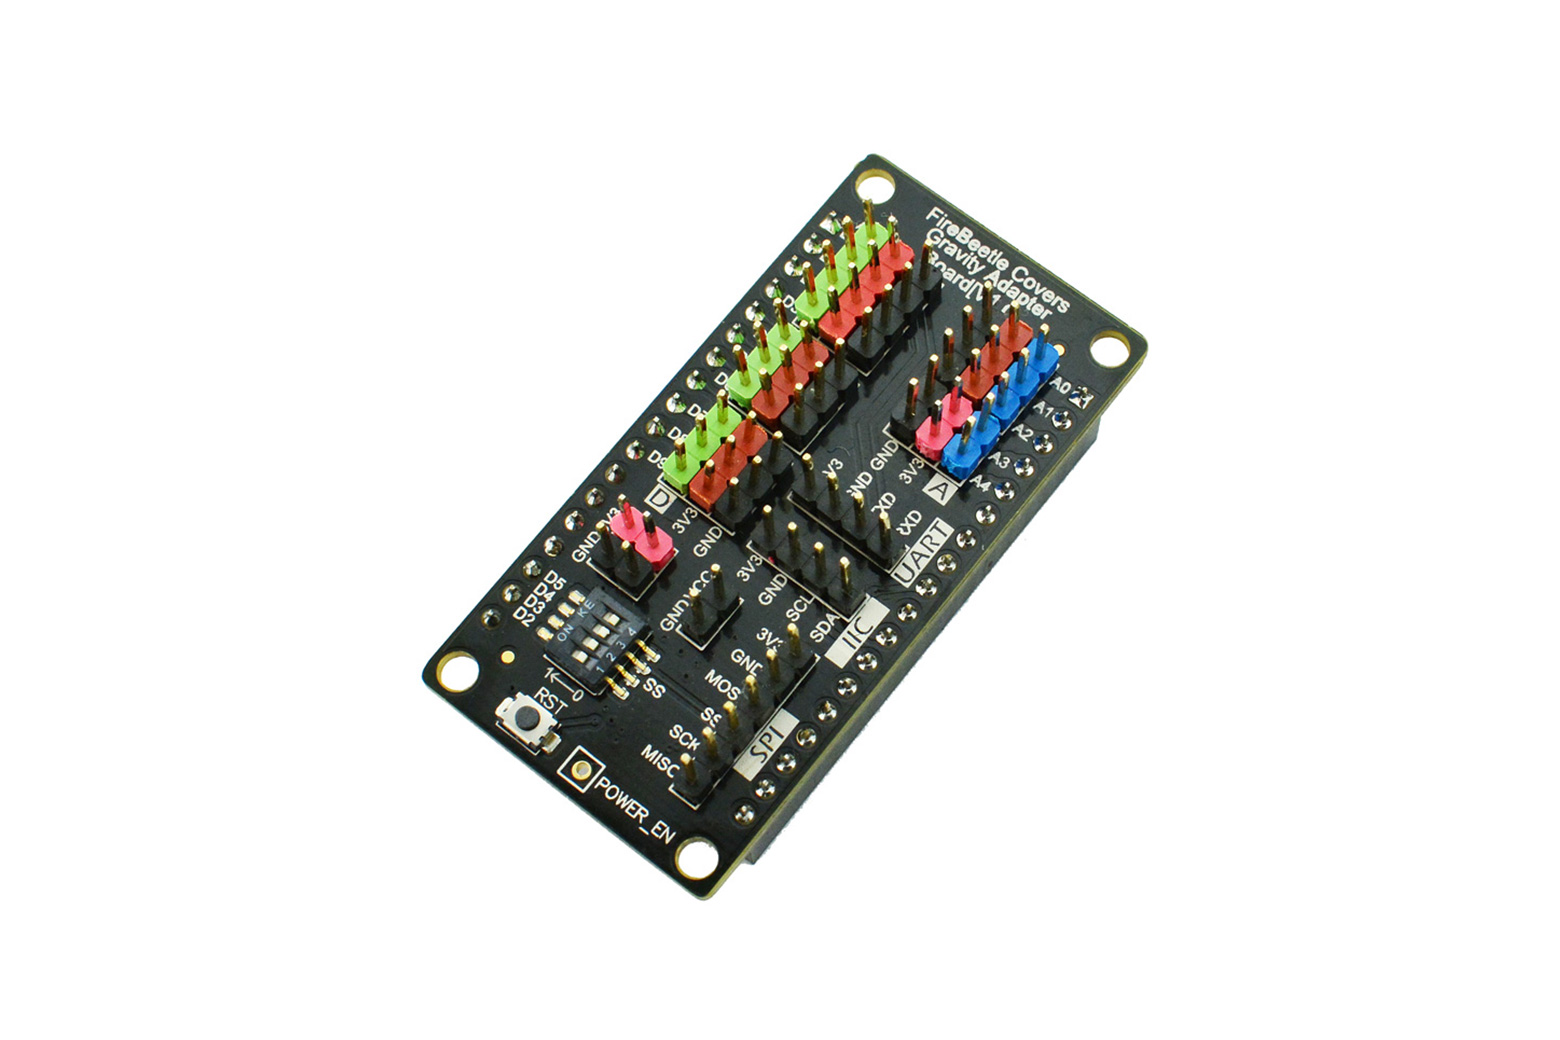
\includegraphics[height=2.4cm, keepaspectratio]{figures/GravityIOExpansionShield_FirebeetleCovers.jpg}
        \caption{I/O Expansion Shield~\cite{dfrobot_gravity_shield}}
        \label{fig:GravityShield}
    \end{subfigure}
    \hfill
    \begin{subfigure}[t]{0.3\textwidth}
        \centering
        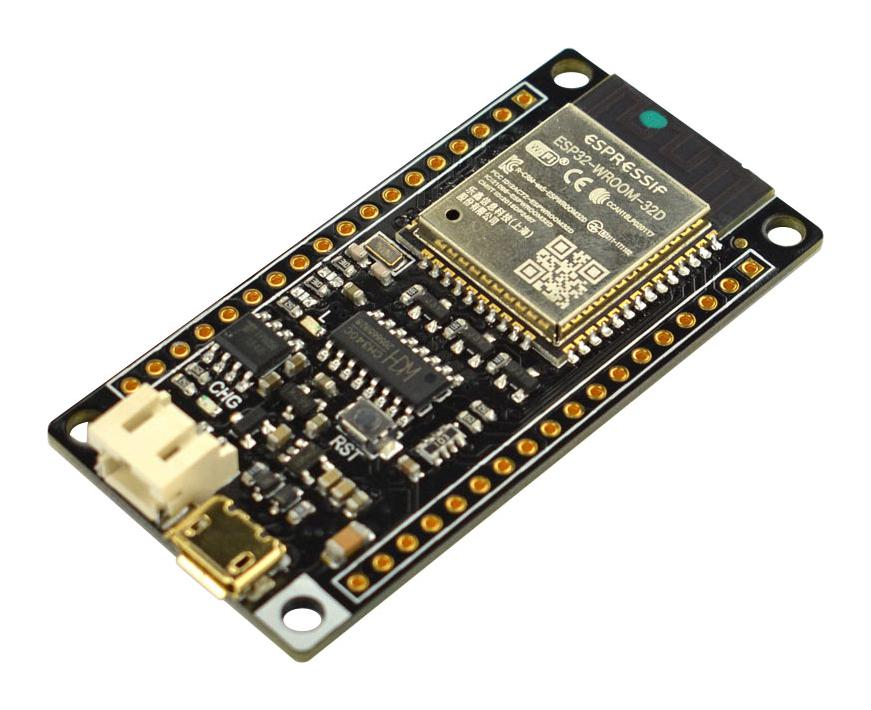
\includegraphics[height=2.4cm, keepaspectratio]{figures/ESP32_Microcontroller.jpg}
        \caption{FireBeetle ESP32~\cite{dfrobot_firebeetle_esp32}}
        \label{fig:ESP32}
    \end{subfigure}
    
    % Row 3
    \hfill
    \begin{subfigure}[t]{0.3\textwidth}
        \centering
        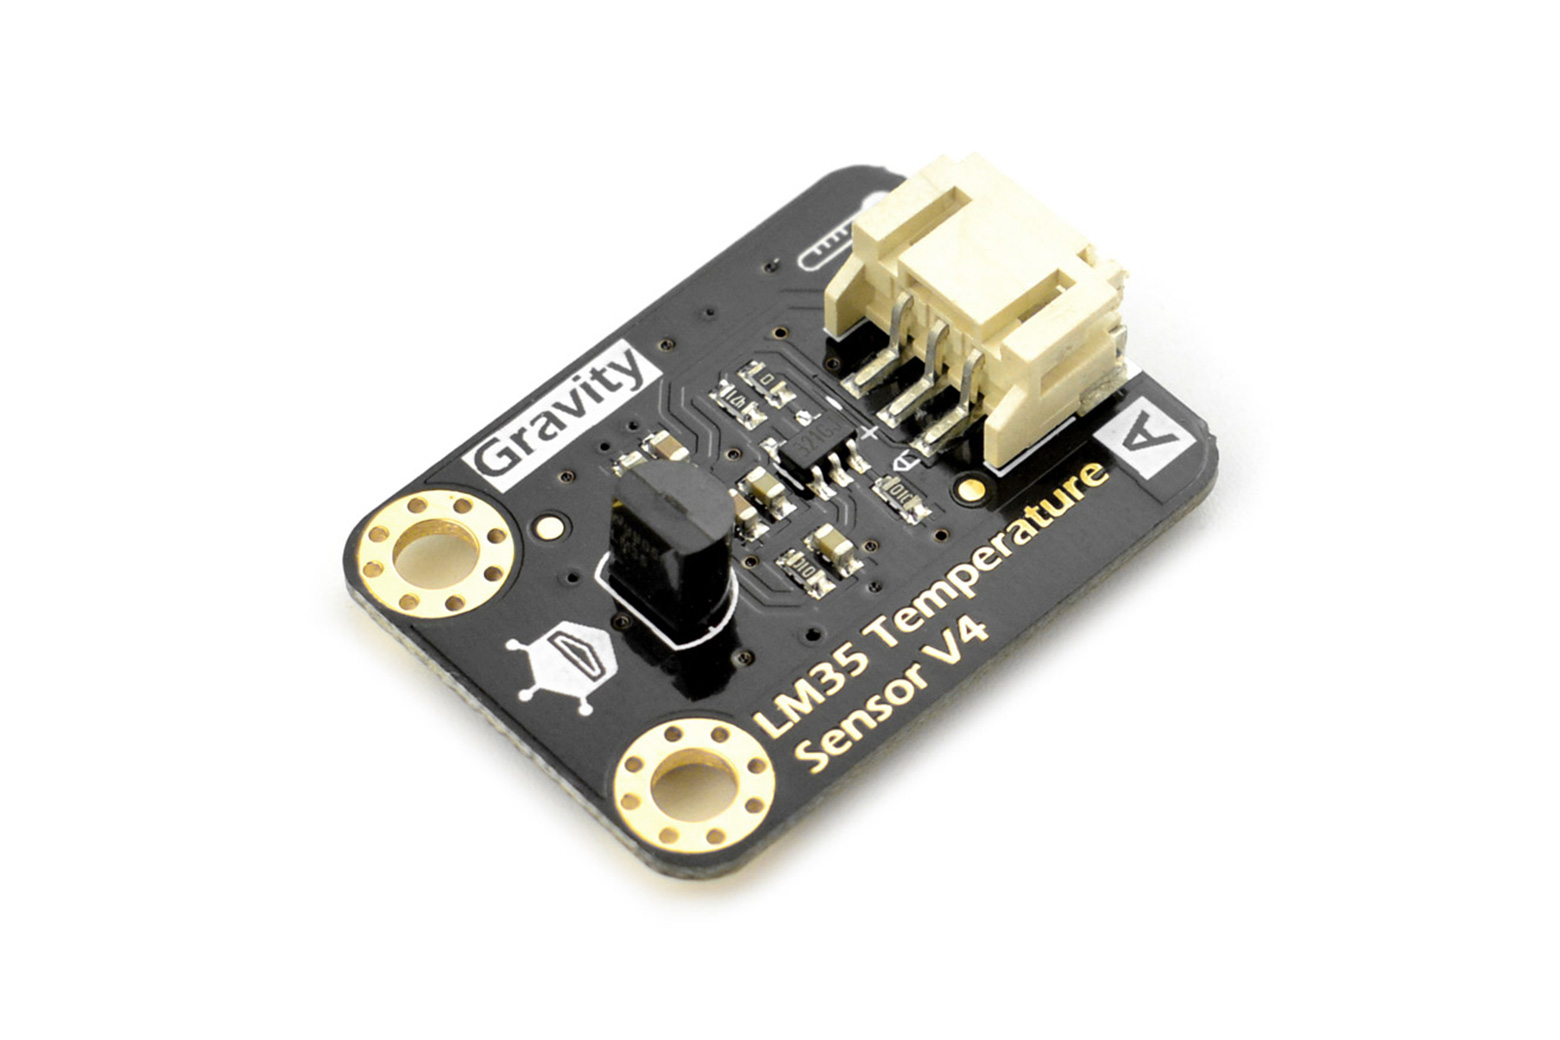
\includegraphics[height=2.4cm, keepaspectratio]{figures/LM35_TemperatureSensor.jpg}
        \caption{LM35 Sensor~\cite{lm35}}
        \label{fig:LM35}
    \end{subfigure}
    \hfill
    \begin{subfigure}[t]{0.3\textwidth}
        \centering
        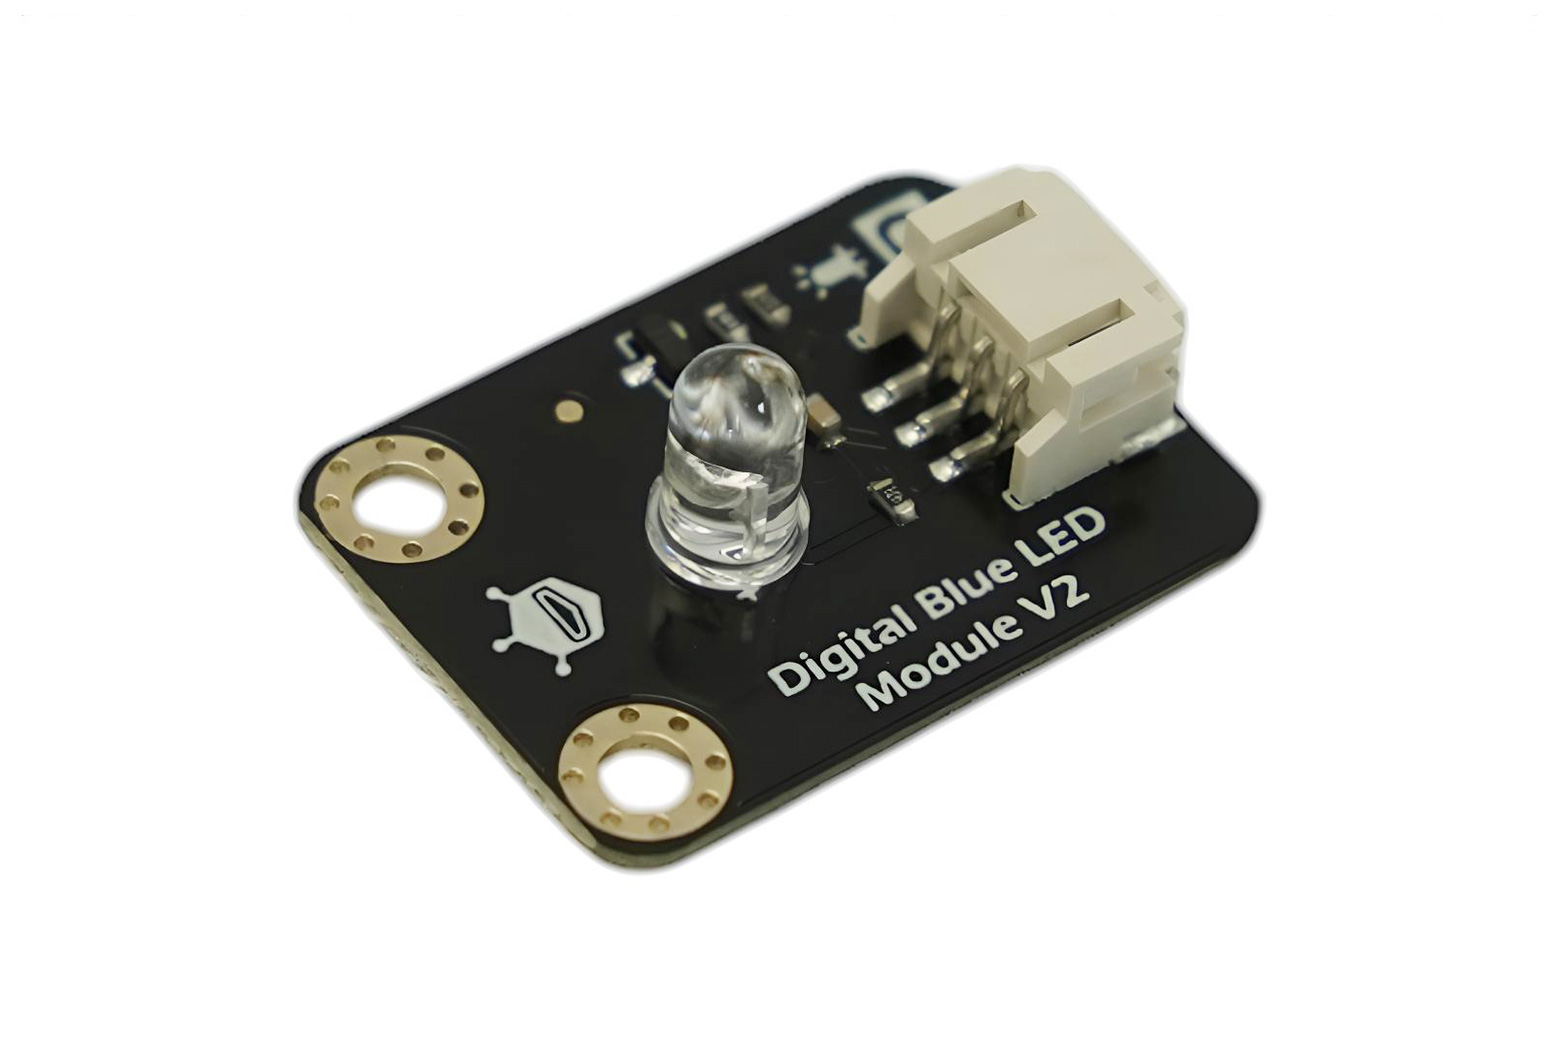
\includegraphics[height=2.4cm, keepaspectratio]{figures/BlueLED.jpg}
        \caption{Blue LED Module~\cite{dfrobot_led_module_dfr0021}}
        \label{fig:LED}
    \end{subfigure}
    \hfill
    \vspace{.5em}
    \caption{Hardware components used in the experimental setup.}
    \label{fig:hardware_components}
\end{figure}


\subsubsection*{Current Measurement Chain (SCT013 + Bias + ADS1115)}

The load current is measured using a non-invasive SCT013 current transformer, enabling galvanic isolation between the mains-powered appliance and the low-voltage measurement electronics. The sensor is clamped around the live conductor supplying the hair dryer, producing a secondary AC current proportional to the primary load current without requiring direct electrical contact.

The secondary output of the SCT013 is converted into a measurable voltage using a burden resistor, after which the signal is conditioned to interface with single-supply digital electronics. Since the sensor output is an AC waveform centered around 0\,V, a midpoint bias network referenced to half of the 3.3\,V supply is applied (1.65\,V). This bias shifts the waveform into the valid input range of the analog-to-digital converter while preserving its amplitude and phase information. Basic passive filtering is included to reduce high-frequency noise and improve signal stability.

The conditioned and biased voltage signal is digitized using an external ADS1115 16-bit analog-to-digital converter. The ADS1115 is configured for single-ended input operation and samples the current measurement signal on channel AIN1 with respect to ground. Compared to the ESP32’s internal ADC, the external ADC provides improved resolution, reduced noise sensitivity, and more repeatable measurements, which is particularly beneficial for low-frequency AC current monitoring.

All components of the current measurement chain operate in the low-voltage domain and share a common ground reference, while the SCT013 ensures electrical isolation from the high-voltage AC circuitry. This architecture allows safe and accurate acquisition of load current data suitable for further processing in software.

\subsubsection*{Temperature Measurement Chain (LM35)}

The outlet air temperature is measured using an LM35 analog temperature sensor, which provides an output voltage linearly proportional to temperature (10\,mV/\textdegree C). The sensor is powered from the 3.3\,V supply and referenced to the common low-voltage ground, ensuring compatibility with the ESP32 analog input range.

The LM35 output is connected directly to an ESP32 ADC input pin, as the sensor’s output voltage remains within safe limits for the microcontroller under the expected temperature range. Due to the analog nature of the signal, wiring between the sensor and the microcontroller was kept short to minimize noise pickup and ensure stable readings.

Physically, the sensor is positioned between the detachable nozzle and the main air outlet of the hairdryer, exposed to the outgoing airflow while avoiding direct contact with heating elements. This placement was determined through iteration: initial attempts to position the sensor outside the nozzle yielded readings that were too low to be useful for safety monitoring, as the airflow had already cooled significantly by that point. Moving the sensor to the position between the nozzle and the main outlet provides a representative measurement of operating temperature with acceptable response time, while reducing thermal stress and measurement instability caused by localized hot spots.

Basic validation of the temperature measurement was performed by comparing sensor output against ambient room temperature under no-load conditions and observing expected temperature rises during normal device operation. These checks confirmed correct sensor orientation, electrical connection, and thermal coupling prior to integration with the control logic.

\begin{figure}[H]
  \centering
  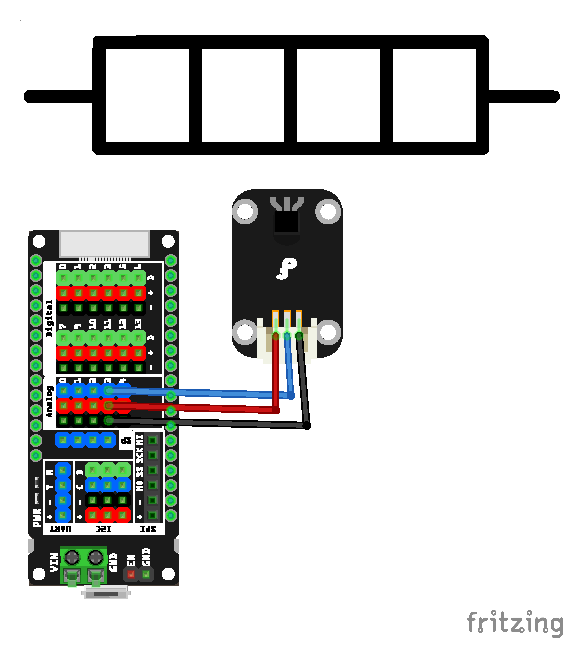
\includegraphics[width=0.6\linewidth]{figures/LM35_TemperatureChain_Schematic.pdf}
  \caption{Close-up schematic of the LM35 temperature measurement chain and ESP32 ADC connection.}
  \label{fig:lm35_chain}
\end{figure}

\subsubsection*{Actuation Hardware (Blue LED / Relay Cutoff)}

System actuation and user feedback are provided through a low-voltage relay and a blue status LED module, both controlled by the ESP32 via digital GPIO pins. The relay enables electrical isolation between the low-voltage control electronics and the mains-powered load, allowing the system to enable or disable the appliance safely.

The relay control input is driven by a dedicated GPIO pin configured as a digital output. The relay module incorporates the required driver and isolation circuitry to interface directly with 3.3\,V logic levels, ensuring reliable switching while preventing high-voltage transients from propagating to the microcontroller. The relay contacts are located exclusively on the mains side of the circuit.

Visual system feedback is provided by a DFRobot digital blue LED module connected to a separate GPIO pin. The module integrates the LED and its current-limiting circuitry on-board, allowing it to be driven directly from a 3.3\,V digital output without the need for an external series resistor. This simplifies wiring and reduces component count while maintaining safe operating conditions. The LED operates entirely within the low-voltage domain and provides a clear indication of system state (e.g., relay enabled or disabled).

\begin{figure}[H]
  \centering
  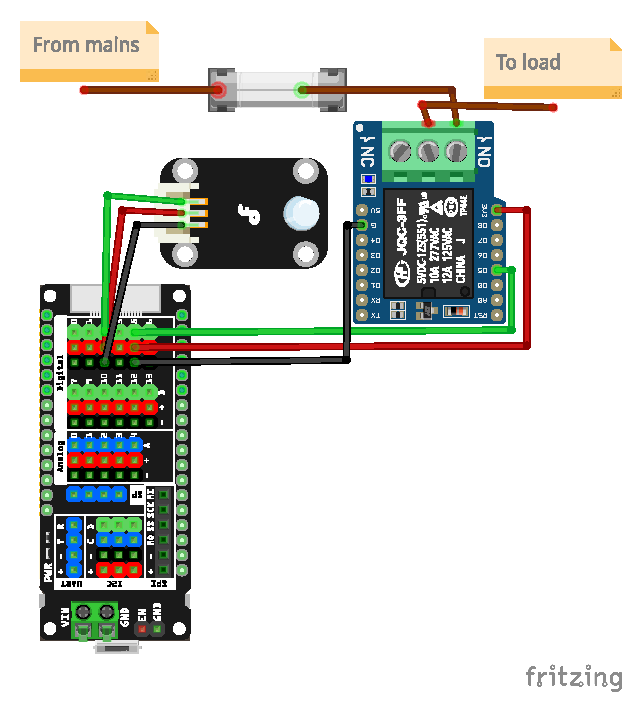
\includegraphics[width=0.6\linewidth]{figures/Actuation_LED_Relay_Schematic.pdf}
  \caption{Close-up schematic of the relay cutoff and blue LED module actuation circuitry controlled by the ESP32.}
  \label{fig:actuation_chain}
\end{figure}


\subsection{Hardware Build Photos}
\begin{figure}[H]
  \centering
  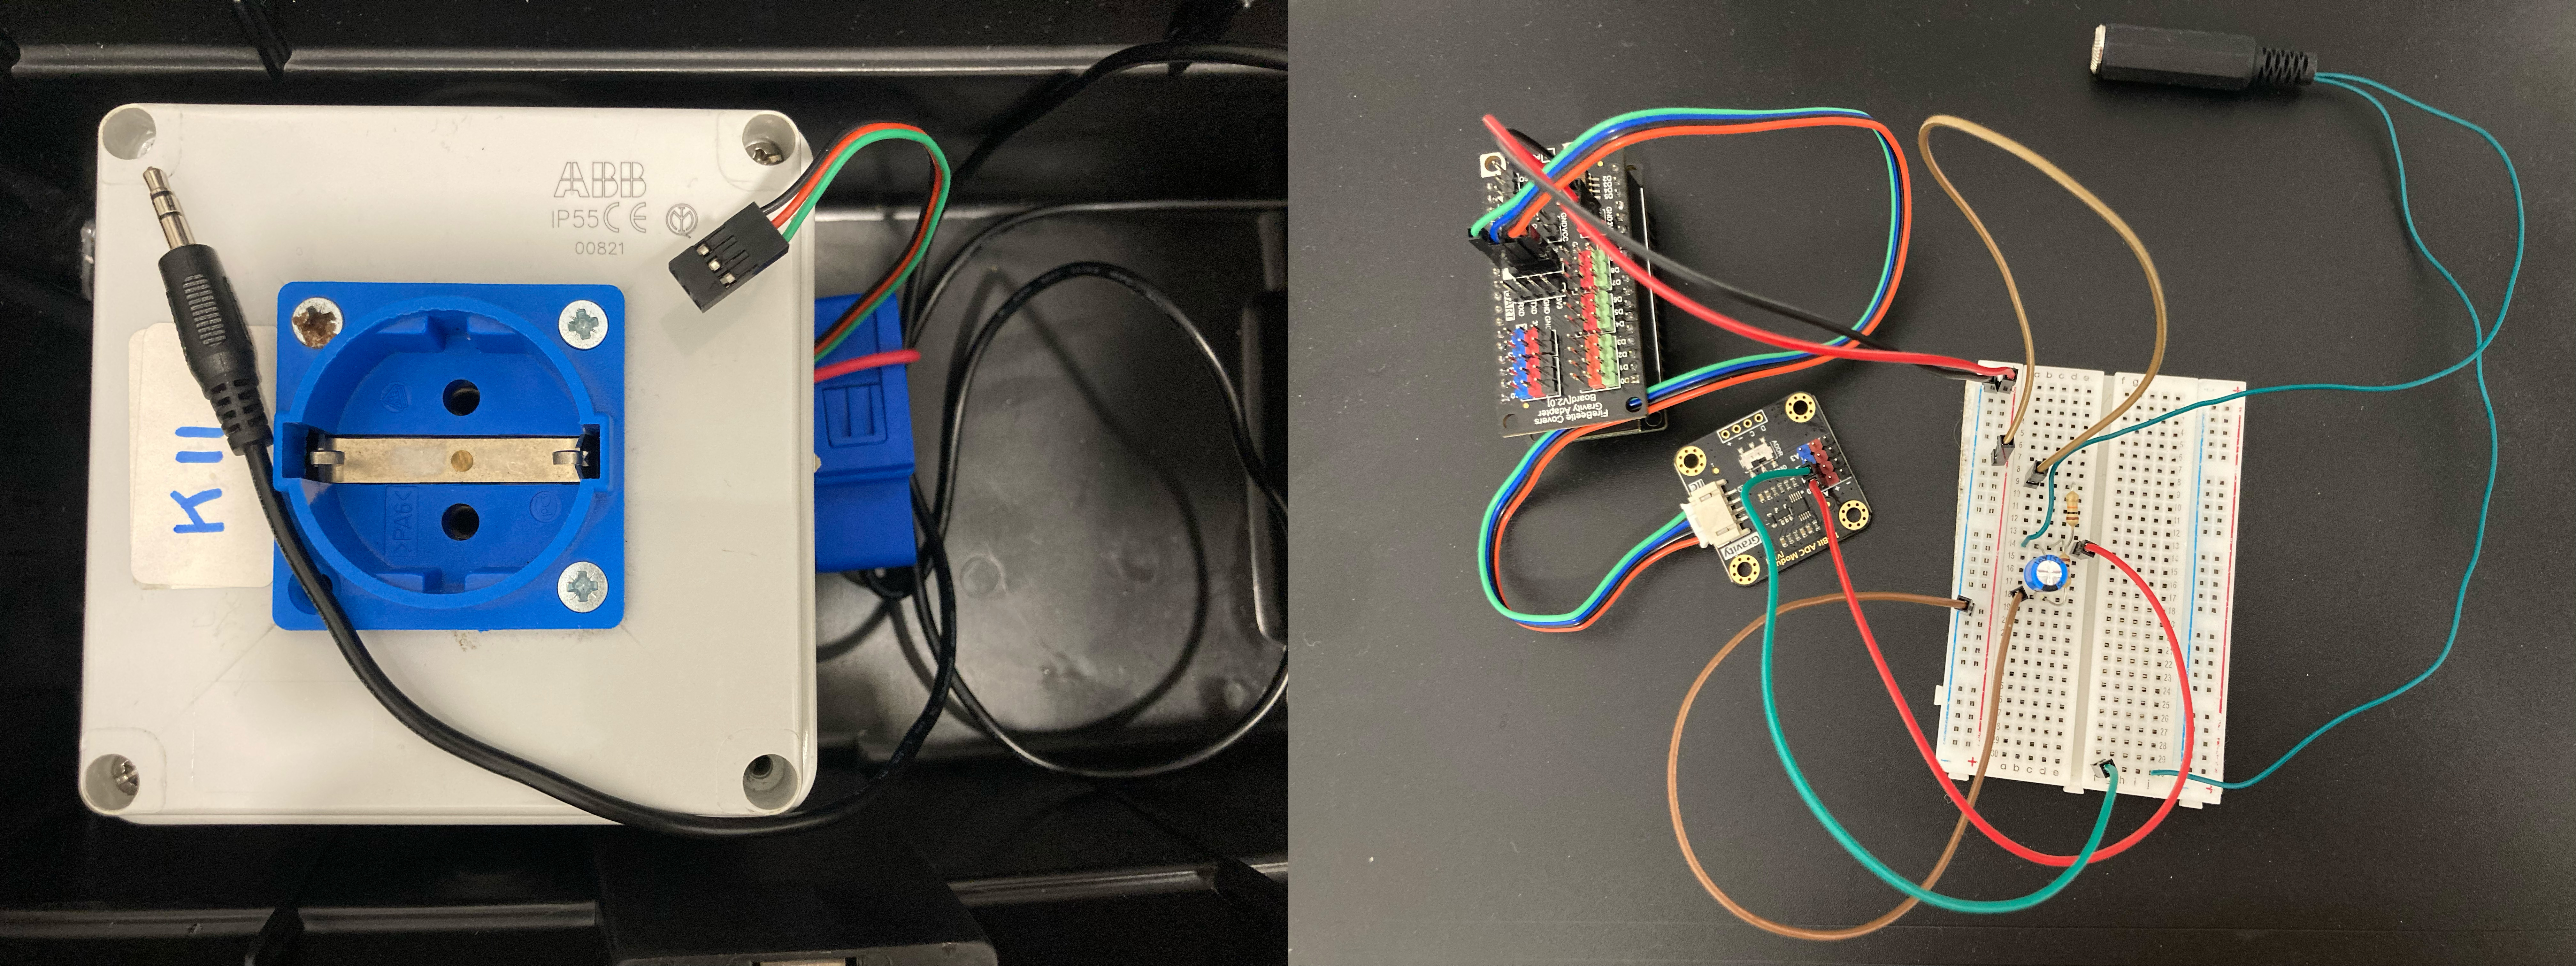
\includegraphics[width=0.6\linewidth]{figures/IMG_6610.jpg}
  \caption{Hardware: AC side and DC side.}
\end{figure}
\begin{figure}[H]
  \centering
  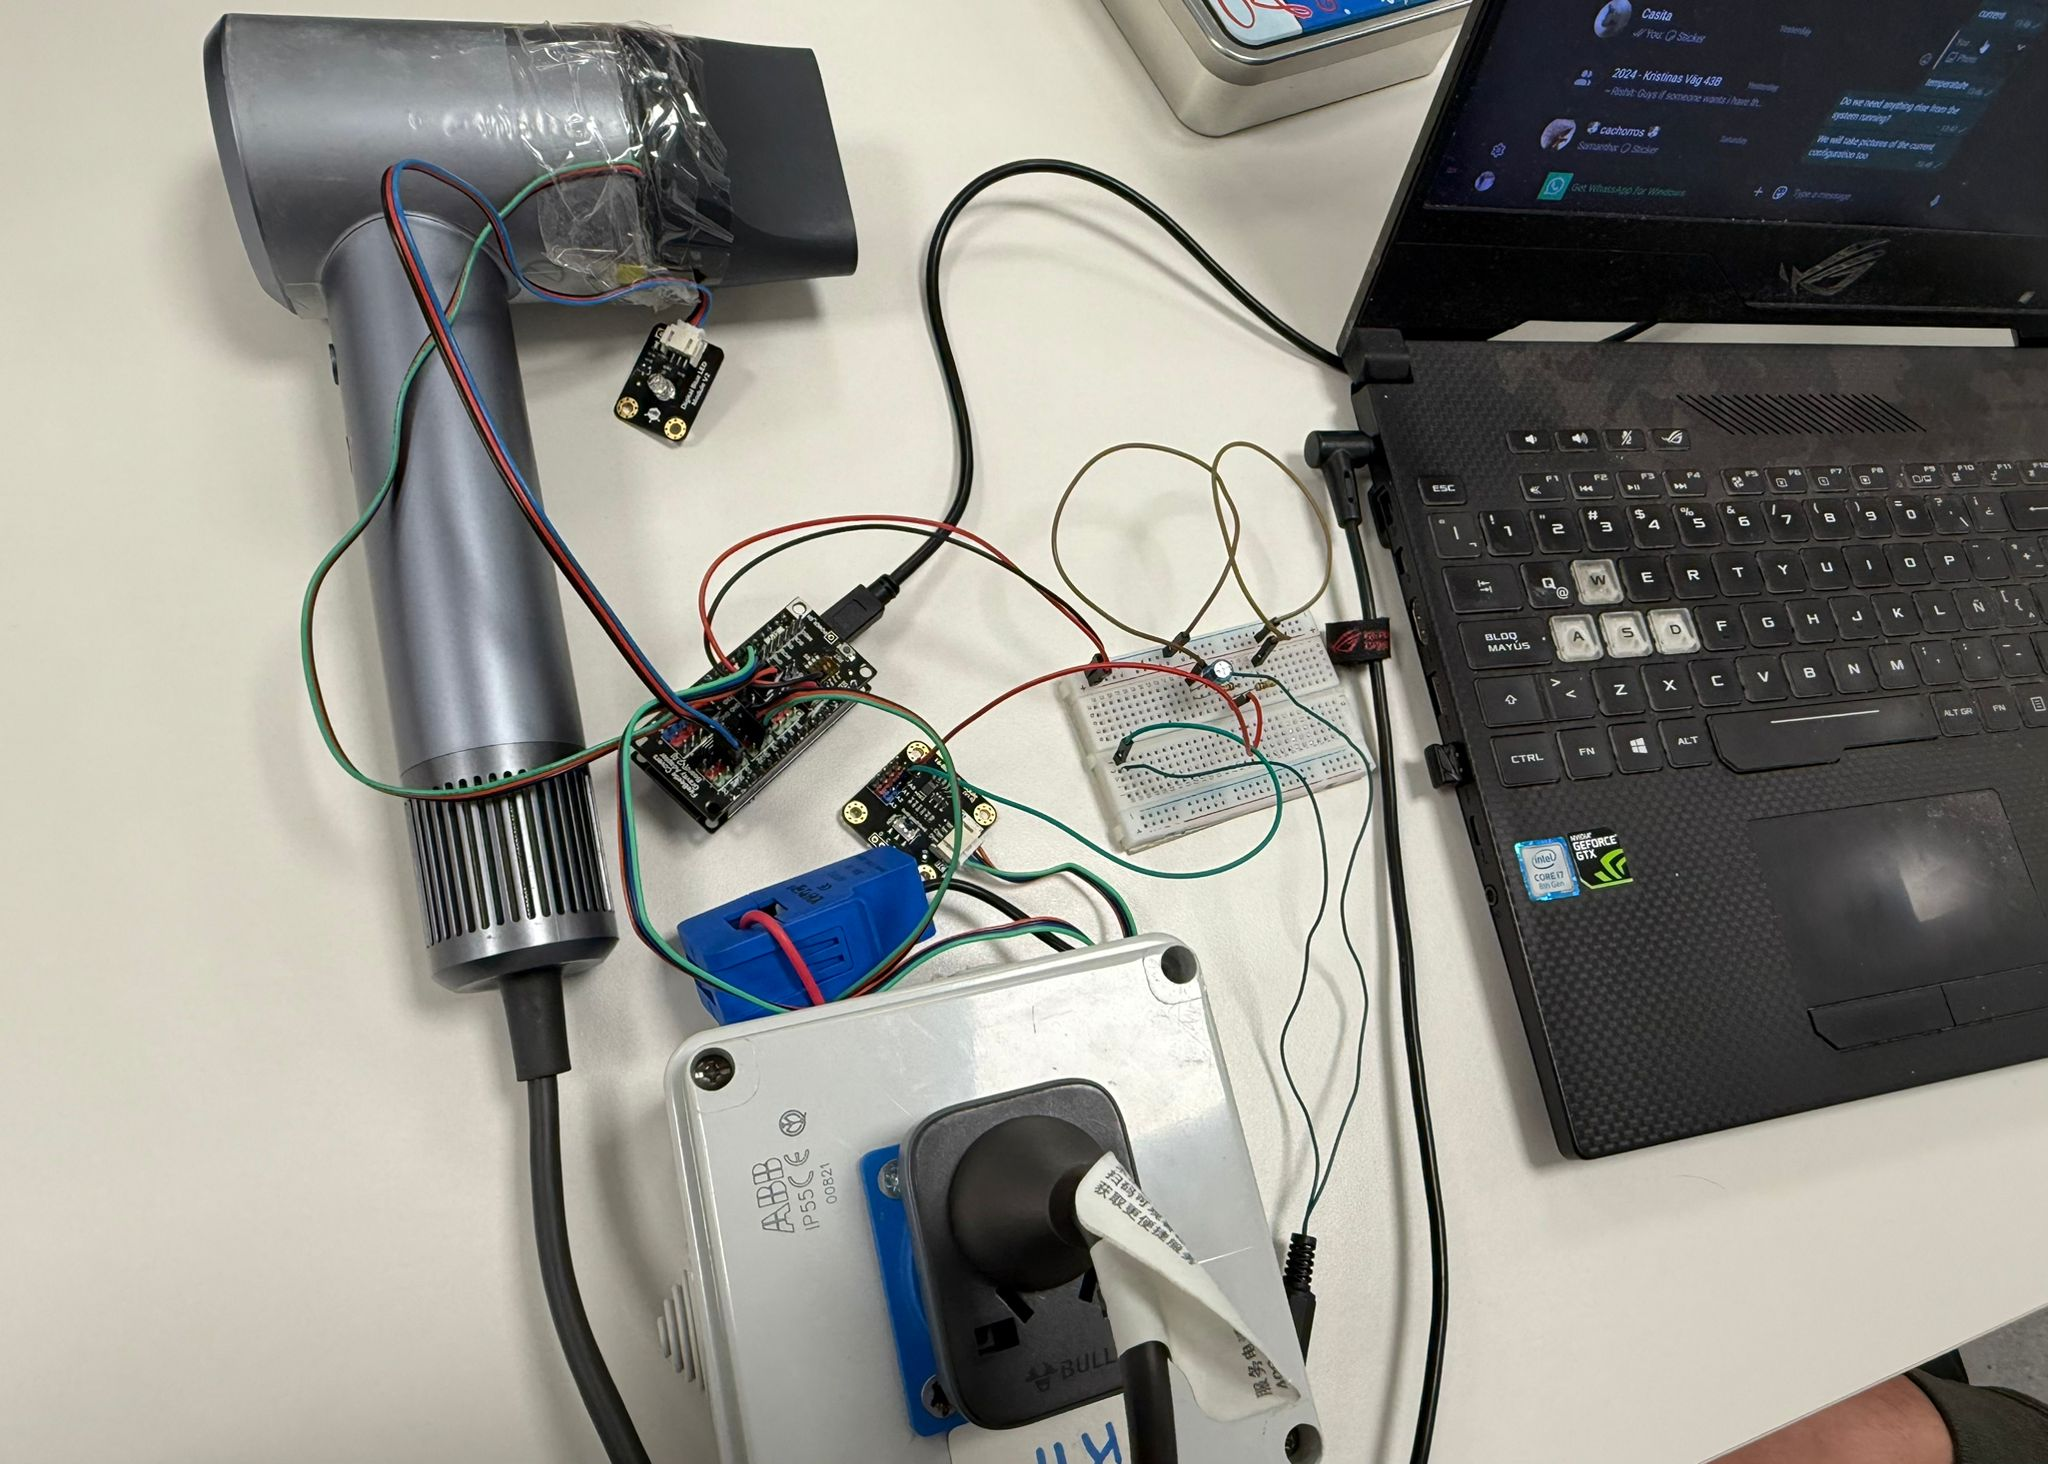
\includegraphics[width=0.85\linewidth]{figures/FullSetup.jpeg}
  \caption{Hardware: full setup.}
\end{figure}

% ==================================================
\newpage
\section{Prototype Development --- Software}

\begin{figure}[H]
  \centering
  \begin{tikzpicture}[
    node distance=1.5cm and 2cm,
    box/.style={rectangle, draw, fill=blue!10, text width=3cm, align=center, rounded corners, minimum height=1cm},
    api/.style={rectangle, draw, fill=green!10, text width=2.8cm, align=center, rounded corners, minimum height=1cm},
    sensor/.style={rectangle, draw, fill=orange!10, text width=2.5cm, align=center, rounded corners, minimum height=0.8cm},
    arrow/.style={->, >=stealth, thick},
    dashed_arrow/.style={->, >=stealth, thick, dashed, gray}
  ]

    % Top layer - External APIs
    \node[api] (openmeteo) at (-1.5,0) {Open-Meteo API\\(Weather Data)};
    \node[api] (ree) at (2,0) {REE API\\(Electricity Price)};

    % Second layer - Dashboard (OPTIONAL)
    \node[box, fill=cyan!10, dashed, draw=gray] (dashboard) at (-1.5,-2) {Streamlit\\Dashboard\\(Optional UI)};

    % Terminal Input (Alternative to Dashboard)
    \node[box, fill=yellow!10] (terminal) at (5,-2) {Terminal Input\\(Barcelona, medium, normal)};

    % Third layer - API Layer
    \node[box, fill=green!20] (fastapi) at (0.25,-3.95) {FastAPI\\Protocol API};

    % Fourth layer - Calculation Module
    \node[api] (calculator) at (0.25,-5.75) {Hairdry Protocol\\Calculator};

    % Fifth layer - Main Control
    \node[box, fill=blue!20, text width=3.5cm] (mainpy) at (2,-7.6) {Main Control\\Safety Strategy};

    % Bottom layer - Arduino (or Simulation)
    \node[box, fill=orange!20] (arduino) at (2,-9.5) {ESP32 Arduino\\(or Simulation)};

    % Sensors
    \node[sensor] (temp) at (-2,-11) {LM35\\Temp Sensor};
    \node[sensor, text width=2.8cm] (current) at (6.5,-11) {SCT013\\Current Sensor};

    % Actuator
    \node[sensor, fill=red!10] (relay) at (2,-11.5) {Relay\\Load Control};

    % Arrows - Data flow
    \draw[dashed_arrow] (openmeteo) -- node[left, font=\tiny, text=gray] {optional} (dashboard);
    \draw[dashed_arrow] (ree) -- (dashboard);
    \draw[arrow] (openmeteo) to[out=-20, in=90] (mainpy);
    \draw[arrow] (ree) to[out=-50, in=90] (mainpy);
    \draw[dashed_arrow] (dashboard) -- node[left, font=\tiny, text=gray] {user inputs} (fastapi);
    \draw[arrow] (terminal) -- node[right, font=\tiny] {location, hair type} (mainpy);
    \draw[arrow] (fastapi) -- node[left, font=\tiny] {GET /protocol} (calculator);
    \draw[arrow] (calculator) -- (mainpy);
    \draw[arrow] (mainpy) -- node[right, font=\tiny] {Serial or simulated} (arduino);
    \draw[arrow] (arduino) -- node[left, font=\tiny] {sensor data (5s)} (mainpy);
    \draw[arrow] (temp) -- (arduino);
    \draw[arrow] (current) -- (arduino);
    \draw[arrow] (arduino) -- node[left, font=\tiny] {H/L commands} (relay);

  \end{tikzpicture}
  \caption{Software schematic.}
  \label{fig:software_schematic}
\end{figure}

\subsection{Software Architecture}

The software \cite{acesschematic} operates in two distinct modes with six primary modules:

\begin{longtable}{|L{0.3\textwidth}|p{0.65\textwidth}|}
\caption{System Components and Descriptions}
\label{tab:system_components} \\
\hline
\textbf{Component} & \textbf{Description} \\
\hline
\endfirsthead
\hline
\textbf{Component} & \textbf{Description} \\
\hline
\endhead
\hline
\endfoot
\hline
\endlastfoot
Operation Modes & The system supports both \emph{standalone terminal mode} (default) and \emph{dashboard-assisted mode}. In standalone mode, executed via \texttt{run\_integrated.bat} or direct Python invocation, users provide inputs through terminal prompts (location, hair type, porosity), and the main control system directly fetches weather and electricity data from external APIs with built-in fallback values (Barcelona, medium hair, normal porosity). In dashboard mode, launched via \texttt{run.bat}, a Streamlit web interface provides graphical input and visualization while the same backend services handle protocol generation and safety monitoring. Both modes share identical protocol calculation and safety enforcement logic, differing only in user interface presentation. \\
\hline
ESP32 Arduino Firmware (\texttt{Integrated\_Project.ino}) & Implements the lowest-level hardware interface, reading analog sensors through an ADS1115 16-bit ADC for current measurement and the ESP32's built-in ADC for temperature. The firmware samples current at 1 kHz to calculate RMS values over 20 ms intervals, then averages 250 RMS samples to produce one filtered output every 5 seconds. It communicates via serial at 115200 baud, responding to relay control commands (`H' for high/on, `L' for low/off) and transmitting sensor readings in the format: \texttt{Temperature: XX.XX | Current: X.XXXXX}. \\
\hline
Main Control System (\texttt{Integrated\_Project.py}) & Serves as the central coordinator, managing three key responsibilities: Serial communication with the ESP32 through the \texttt{SerialBoard} class; Hairdry Protocol acquisition from the local API with user-specific parameters; Real-time safety monitoring by feeding sensor data to the \texttt{SafetyStrategy} module. It runs a continuous monitoring loop synchronized to the Arduino's 5-second output interval, checking for threshold violations and commanding relay shutdown when safety limits are exceeded. This module implements \emph{simulation mode}: when Arduino connection fails, it generates synthetic sensor data (temperature ramping 65-89°C, current cycling 5-7 A) with realistic 5-second timing, enabling complete software testing without physical hardware. The simulation follows the same code paths as real operation, validating protocol logic, safety enforcement, and user interaction flows. \\
\hline
Protocol API (\texttt{mock\_protocol\_api.py}) & Provides a RESTful interface via FastAPI at port 8000, accepting query parameters including room temperature, humidity, hair type, porosity, towel-dry level, time priority, and safety thresholds. It delegates calculation logic to the protocol calculator module and returns a JSON response specifying sensor-specific thresholds (temperature and current) with corresponding duration limits. \\
\hline
Protocol Calculator (\texttt{protocol\_calculator.py}) & Implements the core recommendation engine, calculating optimal drying parameters based on environmental factors and user characteristics. It computes a drying power index from temperature and humidity, determines appropriate heat settings (Low/Medium/High), estimates bulk and finish phase durations, and generates safety protocol thresholds. It also interfaces with external APIs to fetch real-time room conditions from Open-Meteo and electricity prices from the Spanish REE API or regional fallback values. \\
\hline
Safety Strategy Module (\texttt{safety\_strategy.py}) & Monitors sensor readings against protocol thresholds with duration-based violation detection. For each condition (temperature and current), it starts a timer when thresholds are exceeded and triggers shutdown if conditions persist, and hysteresis is implemented by resetting timers when values normalize, preventing false triggers. \\
\hline
Streamlit Dashboard (\texttt{StreamlitDashboard.py}) & Provides a web-based user interface for inputting location, hair characteristics (type and porosity), and viewing personalized drying protocols. It displays environmental conditions, recommended drying phases (towel-dry, optional air-dry, bulk heat, and finish), total time estimates, and energy cost analysis across multiple time-priority and towel-dry level combinations. The dashboard visualizes cost trade-offs through interactive charts, acting as a demonstration for how a user interface may help users select optimal drying strategies. \\
\hline
\end{longtable}

\subsection{Data Streams and Sources}

The system integrates multiple external and internal data sources with specific update frequencies and failure handling:

\begin{longtable}{|L{0.3\textwidth}|p{0.65\textwidth}|}
\caption{Data Streams and Sources}
\label{tab:data_streams} \\
\hline
\textbf{Data Source} & \textbf{Description} \\
\hline
\endfirsthead
\hline
\textbf{Data Source} & \textbf{Description} \\
\hline
\endhead
\hline
\endfoot
\hline
\endlastfoot
Open-Meteo Weather API & Provides current temperature and relative humidity for specified locations. Two endpoints are used: geocoding API converts location names to coordinates, and forecast API returns weather data with temperature and humidity fields. Both dashboard and main control system access this API, enabling standalone operation. Requests timeout after 5 seconds with fallback to Barcelona coordinates or default values (20°C, 60\% humidity) on failure. \\
\hline
REE Electricity Price API & Delivers Spanish real-time electricity prices with hourly granularity. The system queries current hour's price in €/MWh and converts to €/kWh. Both UI modes access this via unified function. For non-Spanish locations or API failures, a regional price map provides fallback values ranging from 0.14 to 0.35 €/kWh. \\
\hline
Arduino Sensor Data Stream & Transmits temperature and current readings every 5 seconds over serial. Temperature measurements use the LM35's linear 10 mV/°C characteristic: $T = V \times 100$, where $V$ is the ADC voltage. Current measurements undergo two-stage filtering: RMS calculation over 20 ms windows (matching AC power frequency), then averaging 250 RMS samples for noise reduction. The 5-second interval balances responsiveness with computational efficiency, as the ESP32 performs $250 \times 20 = 5000$ ms of RMS integration per output. In \emph{simulation mode} (triggered when \texttt{SerialBoard.connect()} fails), the main control system generates synthetic sensor data matching the same timing and format: temperature values cycle from 65°C to 89°C with random noise ($\pm 1^\circ C$), and current cycles from 5.0 to 7.0 A with noise ($\pm 0.1$ A). This simulation maintains the 5-second update cadence and identical data format (\texttt{Temperature: XX.XX | Current: X.XXXXX}), enabling full protocol validation, threshold testing, and UI verification without physical hardware. \\
\hline
Serial Communication & Uses a simple ASCII format for bidirectional communication at 115200 baud. Commands from Python to Arduino consist of single characters (`H' for relay on, `L' for relay off, `PING' for handshake verification). Sensor data from Arduino follows the template \texttt{Temperature: XX.XX | Current: X.XXXXX}, parsed by splitting on the pipe character and extracting float values after colons. The Python \texttt{SerialBoard} class buffers incoming data in a background thread, updating \texttt{latest\_temp} and \texttt{latest\_current} attributes that the main control loop reads. \\
\hline
\end{longtable}

\subsection{Control and Recommendation Logic}

Three-tier safety thresholds with duration-based triggering and hysteresis are implemented:

\begin{longtable}{|L{0.3\textwidth}|p{0.65\textwidth}|}
\caption{Control and Recommendation Logic Components}
\label{tab:control_logic} \\
\hline
\textbf{Component} & \textbf{Description} \\
\hline
\endfirsthead
\hline
\textbf{Component} & \textbf{Description} \\
\hline
\endhead
\hline
\endfoot
\hline
\endlastfoot
Temperature Threshold Monitoring & The protocol specifies a maximum temperature (e.g., 38°C measured at sensor location) and total duration limit based on calculated drying time. When sensor temperature exceeds threshold, \texttt{SafetyStrategy} records the violation timestamp. If temperature remains elevated for the full duration (e.g., total drying time of 4.2 minutes = 252 seconds in demo mode), the system triggers shutdown with the message "You used too long the total hairdrying duration." If temperature drops below threshold before duration expires, the timer resets, implementing hysteresis to prevent oscillation. \\
\hline
Current Threshold Monitoring & High current indicates high heat mode usage on the hairdryer. The system monitors for sustained current above threshold (e.g., 5.0 A) for the bulk phase duration (e.g., 2.4 minutes). This prevents prolonged high-heat exposure that could damage hair, triggering shutdown with "You used too long the high heat mode in your hairdryer" when violated. The duration corresponds to the bulk drying phase, allowing sufficient time for the high-heat portion while preventing overuse. \\
\hline
Maximum Runtime Limit & A failsafe 30-minute (1,800,000 ms) absolute runtime limit prevents indefinite operation regardless of sensor readings. This protects against sensor failures or unexpected usage patterns. In demo mode, all durations divide by 10 for faster testing (e.g., 30 minutes becomes 3 minutes). \\
\hline
Hysteresis Implementation & The \texttt{SafetyStrategy.check\_violations()} method maintains per-condition state including \texttt{triggered\_at} timestamps. Violations only count when continuously exceeding thresholds for full durations. Dropping below threshold at any point resets the timer to \texttt{None}, requiring a fresh sustained violation to trigger shutdown. This design prevents false alarms from brief temperature spikes or momentary high-heat bursts during normal hair manipulation. \\
\hline
Recommendation Engine & The protocol calculator determines heat settings through a multi-factor index. Starting with a hair-type baseline (fine=0, medium=1, thick=2), it adjusts for porosity (low +1, high -1), environmental drying power (DP $< 0.6$ adds +1, DP $> 1.2$ subtracts -1), and time priority (scaled by $0.5 \times (\text{priority} - 0.5)$). The final heat index, clamped to 0-2, maps to Low (50-60°C), Medium (70-80°C), or High (90-100°C) settings. Drying time calculation begins with a base bulk time: $t_{\text{bulk}} = \left(2 + \frac{\text{towel\_level} - 50}{25}\right) \times k_{\text{hair}} \div \left(0.5 + 0.5 \times \text{DP}\right) \div \left(1 + 0.3 \times \text{priority}\right)$ where $k_{\text{hair}} = \{0.7, 1.0, 1.4\}$ for fine/medium/thick hair. The finish time follows a similar formula with different coefficients. For favorable conditions (temp $\geq 18$°C, humidity $< 75\%$, DP $\geq 0.5$, priority $\leq 0.7$), the system recommends hybrid drying: 10-30 minutes of air drying followed by reduced blow-dry times (bulk $\times 0.6$, finish $\times 0.7$). \\
\hline
\end{longtable}

\subsection{Details of Key Communication Patterns}

\textbf{Multi-Service Launcher Architecture:} The \texttt{run.bat} script orchestrates three independent services: FastAPI protocol server (port 8000), Streamlit dashboard (port 8501), and main control system with serial connection. Services launch sequentially with configurable delays to ensure dependencies initialize. The script supports optional ngrok tunneling via \texttt{--ngrok} for remote access, dynamically setting environment variables (\texttt{API\_URL}, \texttt{DASHBOARD\_URL}) that the control system reads. For standalone operation, \texttt{run\_integrated.bat} bypasses dashboard and API, launching only the main control script. This provides protocol data via local FastAPI or falls back to hardcoded defaults if unreachable.

\textbf{Automatic Port Discovery:} The \texttt{SerialBoard} class iterates through all available ports, attempting connection to each until successful. For each port, it opens the connection, waits 2 seconds for ESP32 initialization, attempts handshake, and moves to the next port on failure. This eliminates manual configuration.

\textbf{Threaded Sensor Reading:} A daemon thread runs \texttt{read\_sensor\_data()} continuously, parsing incoming serial lines and updating \texttt{latest\_temp} and \texttt{latest\_current} attributes. The main control loop reads these attributes every 5 seconds, decoupling sensor I/O from safety logic. Thread synchronization relies on Python's GIL, as float assignments are atomic operations.

\textbf{Demo Mode Acceleration:} Setting \texttt{DEMO\_MODE = 1} divides all protocol durations by 10 before sending to \texttt{SafetyStrategy}, allowing rapid testing (e.g., 4-minute protocols become 24 seconds). Critically, this only affects safety timeout durations, not the Arduino's sensor sampling or output rate, maintaining realistic sensor data flow during accelerated testing.

\begin{figure}[H]
  \centering
  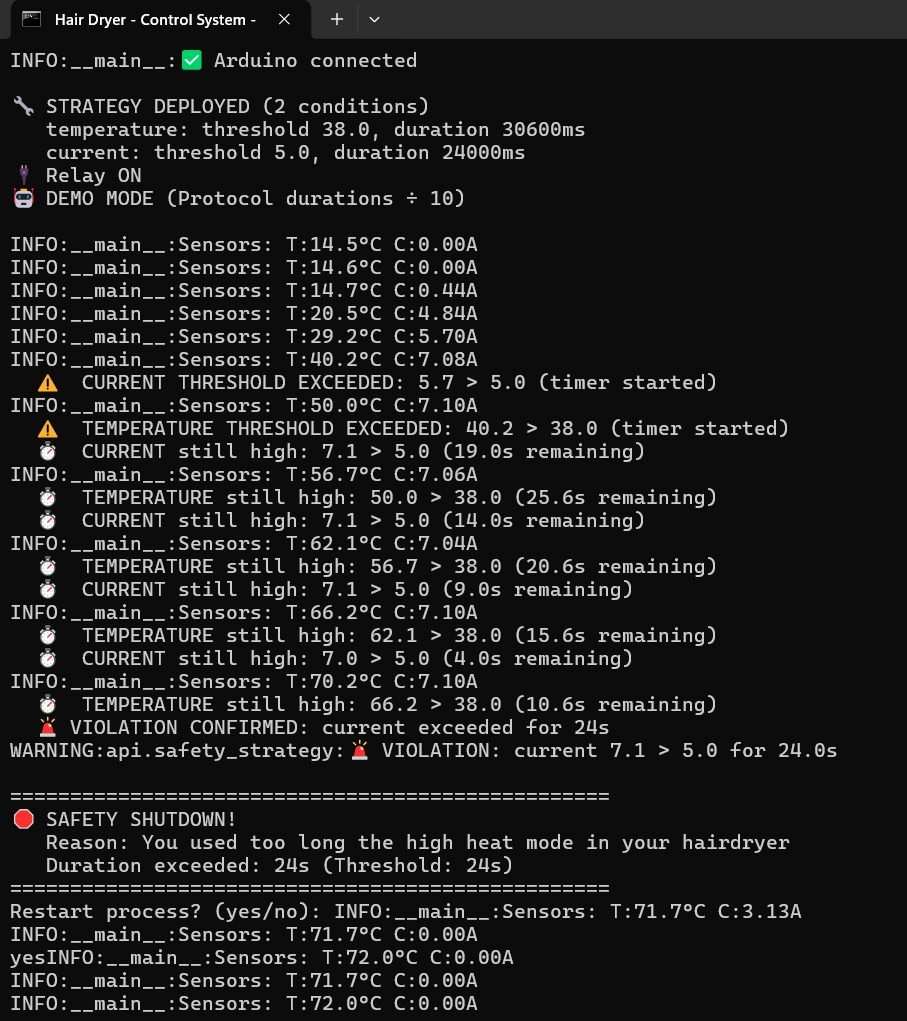
\includegraphics[width=0.6\linewidth]{figures/logging.jpg}
  \caption{Example UI/logging screenshot.}
\end{figure}

% ==================================================
\newpage
\section{Testing and Validation Iterations}

\begin{figure}[H]
  \centering
  \begin{tikzpicture}[
    node distance=0.8cm,
    phase/.style={rectangle, draw, fill=blue!15, text width=2.8cm, align=left, rounded corners, minimum height=0.7cm, font=\footnotesize},
    issue/.style={rectangle, draw, fill=red!15, text width=2.8cm, align=left, rounded corners, minimum height=0.7cm, font=\footnotesize},
    fix/.style={rectangle, draw, fill=green!15, text width=2.8cm, align=left, rounded corners, minimum height=0.7cm, font=\footnotesize},
    test/.style={rectangle, draw, fill=orange!15, text width=2.8cm, align=left, rounded corners, minimum height=0.7cm, font=\footnotesize},
    arrow/.style={->, >=stealth, thick}
  ]
    % Timeline axis
    \draw[thick, ->] (0,0) -- (14,0) node[right, font=\small] {Time};

    % Month labels
    \node[below, font=\scriptsize] at (1.5,-0.3) {Early Oct};
    \node[below, font=\scriptsize] at (4,-0.3) {Mid Oct};
    \node[below, font=\scriptsize] at (6.5,-0.3) {Late Oct};
    \node[below, font=\scriptsize] at (9,-0.3) {Nov};
    \node[below, font=\scriptsize] at (11.5,-0.3) {Dec};

    % Events - staggered vertically for readability
    % Early October
    \node[test] (test1) at (1.5,2.8) {Initial component testing};
    \node[issue] (issue1) at (1.5,1.5) {Temp sensor readings too low (external placement)};

    % Mid October
    \node[fix] (fix1) at (4.3,4) {Oct 15: Sensor moved between nozzle \& outlet};
    \node[issue] (issue2) at (4.3,2.8) {Noisy current measurements};
    \node[issue] (issue3) at (4.3,1.8) {RMS calculation errors};
    \node[fix] (fix2) at (4.3,0.8) {Oct 17: RMS formula corrected};

    % Late October
    \node[fix] (fix3) at (7.2,3.6) {Oct 17: Voltage calibration fixed};
    \node[issue] (issue4) at (7.2,2.6) {Averaging accuracy issues};
    \node[fix] (fix4) at (7.2,1.4) {Oct 23: Dynamic counter implemented};

    % November
    \node[test] (test2) at (10,3.6) {Software integration testing};
    \node[fix] (fix5) at (10,2.4) {Nov 27: Temp reading switched to direct ADC};
    \node[fix] (fix6) at (10,1.05) {Nov 29: Safety strategy \& DEMO mode added};

    % December
    \node[issue] (issue5) at (12.5,4.3) {Serial connection failures};
    \node[fix] (fix7) at (12.5,3.1) {Dec 4: Auto port discovery \& simulation mode};
    \node[issue] (issue6) at (12.5,2) {False safety alarms};
    \node[fix] (fix8) at (12.5,0.8) {Dec 15: Thresholds calibrated (80°C, 5A)};

    % Connecting arrows (selected key paths)
    \draw[arrow, dashed, gray] (issue1) -- (fix1);
    \draw[arrow, dashed, gray] (issue2) -- (fix2);
    \draw[arrow, dashed, gray] (issue3) -- (fix2);
    \draw[arrow, dashed, gray] (issue4) -- (fix4);
    \draw[arrow, dashed, gray] (issue5) -- (fix7);
    \draw[arrow, dashed, gray] (issue6) -- (fix8);

  \end{tikzpicture}
  \caption{Timeline of testing activities, identified issues, and implemented mitigations during prototype development (October--December 2025).}
  \label{fig:testing_timeline}
\end{figure}

\subsection{Test Plan}

Testing was conducted incrementally, validating individual components before integration. No external test equipment was used beyond the prototype itself and standard development tools (serial monitor, Python scripts).

\subsubsection*{Component-Level Testing}

\paragraph{Current Sensor (SCT013)}
The current transformer was tested by connecting it to the hairdryer and observing readings at different power settings. Initial tests revealed noisy measurements, leading to implementation of two-stage filtering: 20 ms RMS calculation synchronized to AC frequency, followed by 250-sample moving average producing stable 5-second updates. Values below 0.1 A were clamped to zero to eliminate sensor offset noise.

\paragraph{Temperature Sensor (LM35)}
Temperature measurements were validated by comparing sensor output against ambient room temperature under no-load conditions. During hairdryer operation, the sensor was positioned near the air outlet to observe expected temperature rises. The linear relationship (10 mV/°C) was verified by checking voltage-to-temperature conversion in the ESP32 ADC range.

\paragraph{Relay and LED}
Actuation hardware was tested using simple serial commands (`H' for high, `L' for low) sent from the Python control script. The relay switching was audibly confirmed, and LED visual feedback verified.

\paragraph{Serial Communication}
ESP32-to-Python communication was validated through handshake testing (PING/PONG protocol) and continuous data streaming. The 115200 baud rate provided reliable transmission of the sensor data format: \texttt{Temperature: XX.XX | Current: X.XXXXX}.

\subsubsection*{Software Functionality Testing}

\paragraph{Simulation Mode}
To enable testing without hardware, a simulation mode was implemented that generates synthetic sensor data (temperature cycling 65-89°C, current cycling 5-7 A) with realistic 5-second timing. This allowed validation of protocol logic, safety enforcement, and user interface without requiring the physical prototype.

\paragraph{DEMO Mode}
For accelerated testing, a DEMO\_MODE flag divides all protocol durations by 10, converting 4-minute protocols into 24-second tests. This significantly sped up validation of threshold violations and safety shutdown logic during development.

\paragraph{API Robustness}
External API calls (Open-Meteo weather, REE electricity pricing) were tested with timeout handling and fallback mechanisms. When APIs failed or returned invalid data, the system defaulted to reasonable values (Barcelona coordinates, 20°C, 60\% humidity, €0.26/kWh).

\paragraph{Protocol Calculation}
The hairdry protocol calculator is based on established hair science principles from the literature~\cite{lee_hair_damage}, which demonstrate the relationship between heat exposure, drying time, and hair damage. Implementation and validation of the underlying protocol logic is outside the scope of this project. Instead, testing focused on verifying that the protocol generator correctly processes user inputs (hair type, porosity, environmental conditions) and produces consistent, internally coherent recommendations consistent with the referenced methodology.

\subsubsection*{Integration Testing}

Full system tests were conducted by running the integrated Python script (\texttt{Integrated\_Project.py}) with the ESP32 connected, simulating realistic usage scenarios:
\begin{itemize}
  \item Normal operation: Hairdryer running within safe limits for typical durations
  \item Temperature violation: Exceeding temperature threshold for the protocol duration
  \item Current violation: Running high-heat mode longer than recommended bulk phase
  \item Recovery: Dropping below thresholds before violation duration expires (hysteresis test)
\end{itemize}

The test software in the repository (\texttt{run.bat}, \texttt{run\_integrated.bat}) facilitated these tests by launching services (API, dashboard, main control) and managing their coordination.

\subsection{Calibration Iterations}

\begin{longtable}{|L{0.2\textwidth}|p{0.75\textwidth}|}
\caption{Calibration Iterations and Refinements}
\label{tab:calibration_iterations} \\
\hline
\textbf{Iteration} & \textbf{Details} \\
\hline
\endfirsthead
\hline
\textbf{Iteration} & \textbf{Details} \\
\hline
\endhead
\hline
\endfoot
\hline
\endlastfoot
Temperature Sensor Physical Placement & \textbf{Before:} Positioned outside the detachable nozzle, in free air downstream. \newline \textbf{After:} Relocated between the nozzle and main air outlet. \newline \textbf{Reason:} External placement yielded readings too low for safety monitoring due to cooling by ambient air mixing. The new placement captures representative operating temperatures while avoiding direct heating element contact and maintains sensor durability. \\
\hline
Temperature Sensor Reading Method (Nov 27) & \textbf{Before:} I2C configuration requiring \texttt{config\_i2c\_temp()} calls and ADS1115 channel switching. \newline \textbf{After:} Direct analog reading using \texttt{analogRead(TEMP\_SENSOR\_PIN)} via ESP32 built-in ADC. \newline \textbf{Reason:} LM35 output voltage (0-100 mV for 0-100°C) fits within ESP32 ADC range, eliminating need for external ADC. Reduced sensor reading latency and improved reliability. \\
\hline
RMS Calculation Formula (Oct 17) & \textbf{Before:} Calculated as $\sqrt{\text{quadratic\_sum} / \text{counter}}$, treating sum as simple average of squared values. \newline \textbf{After:} Changed to $I_{\text{RMS}} = \sqrt{f \times S_{\text{RMS}}}$ where $f = 50$ Hz and $S_{\text{RMS}} = \sum i^2(t) \cdot \Delta t$. \newline \textbf{Reason:} Properly accounts for time-domain integration and power frequency synchronization for accurate RMS values. \\
\hline
Current Sensor Voltage Calibration (Oct 17) & \textbf{Before:} Double calibration error: \texttt{v\_sensor = (read\_voltage() - v\_calib) * (v\_sensor - v\_calib)}. \newline \textbf{After:} Single calibration: \texttt{v\_sensor = read\_voltage() - 1.65}, then \texttt{current = 30.0 * v\_sensor}. \newline \textbf{Reason:} SCT013 output biased to 1.65 V (half 3.3 V supply); only one subtraction needed before applying 30 A/V transformer ratio. \\
\hline
Averaging Calculation (Oct 23) & \textbf{Before:} Fixed constant \texttt{sampleAverage} regardless of samples collected. \newline \textbf{After:} Dynamic \texttt{accumulated\_counter}: \texttt{filteredCurrentRms = accumulatedCurrent / accumulated\_counter}. \newline \textbf{Reason:} Using actual count improves accuracy especially during startup when buffer isn't full, and ensures robustness to timing variations. \\
\hline
Safety Strategy Threshold Values (Dec 15) & \textbf{Iteration:} Temperature and current thresholds adjusted to 80°C and 5 A based on observed sensor behavior during operation. \newline \textbf{Reason:} Initial thresholds too conservative, triggering false alarms during normal operation. Calibrated values balance safety enforcement with usability. \\
\hline
Hardware Mode Synchronization (Dec 4) & \textbf{Issue:} Serial connection failures caused crashes instead of graceful fallback to simulation mode. \newline \textbf{Fix:} Enhanced \texttt{SerialBoard.connect()} with automatic port discovery, handshake verification, and explicit simulation mode activation. \newline \textbf{Reason:} Improved development workflow and robustness to serial port issues. \\
\hline
\end{longtable}

\subsection{Failure Modes \& Mitigations}

\begin{longtable}{|L{0.2\textwidth}|p{0.75\textwidth}|}
\caption{Failure Modes and Mitigation Strategies}
\label{tab:failure_modes} \\
\hline
\textbf{Failure Mode} & \textbf{Details} \\
\hline
\endfirsthead
\hline
\textbf{Failure Mode} & \textbf{Details} \\
\hline
\endhead
\hline
\endfoot
\hline
\endlastfoot
Serial Connection Loss & \textbf{Failure:} ESP32 disconnects during operation (USB cable unplugged, port driver issue, ESP32 reset). \newline \textbf{Mitigation:} Automatic port discovery iterates through all available serial ports attempting connection. Simulation mode activates if no hardware found, allowing software to continue testing with synthetic data. \\
\hline
Sensor Disconnection or Invalid Readings & \textbf{Failure:} Temperature or current sensors return invalid values (e.g., negative temperature, implausible current spikes). \newline \textbf{Mitigation:} Current values below 0.1 A are clamped to zero. Simulation mode provides known-good data when hardware fails. Future work could add explicit range checking (e.g., temperature between -10°C and 150°C). \\
\hline
Noisy ADC Measurements & \textbf{Failure:} High-frequency electrical noise from hairdryer motor and heating elements couples into sensor signals. \newline \textbf{Mitigation:} Two-stage filtering: (1) RMS calculation integrates 20 ms (one AC period) to reject transients, (2) 250-sample moving average produces stable 5-second output. Burden resistor and passive RC filtering on SCT013 output further reduce noise. \\
\hline
External API Failures & \textbf{Failure:} Open-Meteo or REE API unreachable (network outage, service downtime, rate limiting). \newline \textbf{Mitigation:} All API calls have 5-second timeouts. Weather API falls back to Barcelona coordinates then to default values (20°C, 60\% humidity). Electricity API uses regional price map for non-Spanish locations, then defaults to €0.26/kWh. \\
\hline
False Safety Alarms & \textbf{Failure:} Brief temperature spikes or momentary high-current bursts trigger safety shutdown during normal hair manipulation. \newline \textbf{Mitigation:} Duration-based threshold enforcement with hysteresis. Violations only trigger after continuously exceeding thresholds for the full protocol duration (e.g., 4.2 minutes for temperature). If sensor readings drop below threshold before duration expires, timer resets, requiring a fresh sustained violation. \\
\hline
Relay Contact Failure & \textbf{Failure:} Relay contacts weld closed (stuck on) or fail open (stuck off). \newline \textbf{Mitigation:} Current sensor provides independent verification of load state. If relay commanded off but current remains high, software can detect mismatch and alert user. Physical relay rated for 10 A at 250 VAC with appropriate safety margin for 7 A hairdryer load. \\
\hline
Maximum Runtime Protection & \textbf{Failure:} Software bug or sensor failure prevents normal shutdown, allowing indefinite operation. \newline \textbf{Mitigation:} Absolute 30-minute (1,800,000 ms) timeout regardless of sensor readings. Acts as failsafe against logic errors or stuck sensors. \\
\hline
\end{longtable}

% ==================================================
\newpage
\section{Results and Conclusion}

\subsection{Performance}

\subsubsection*{Current and Power Measurement Results}

The current measurement subsystem successfully achieved stable and accurate RMS current readings across the full operating range of the Xiaomi hair dryer (0--7 A).

\begin{longtable}{|p{0.28\textwidth}|p{0.25\textwidth}|p{0.38\textwidth}|}
\caption{Current and Power Measurement Results by Operating Mode}
\label{tab:current_power_results} \\
\hline
\textbf{Operating Mode} & \textbf{Current Range (A)} & \textbf{Approximate Power (W at 230 V)} \\
\hline
\endfirsthead
\hline
\textbf{Operating Mode} & \textbf{Current Range (A)} & \textbf{Approximate Power (W at 230 V)} \\
\hline
\endhead
\hline
\endfoot
\hline
\endlastfoot
Low Heat Mode & 2.8--3.5 & 650--800 \\
\hline
Medium Heat Mode & 4.2--5.0 & 950--1,150 \\
\hline
High Heat Mode & 5.8--6.8 & 1,300--1,550 \\
\hline
Cool Shot / Motor Only & 1.2--1.8 & 280--400 \\
\hline
\multicolumn{3}{|p{0.92\textwidth}|}{\textbf{Key Findings:} The measured values align closely with the manufacturer's rated power of 1,600 W, with the discrepancy attributed to voltage fluctuations and device efficiency.} \\
\hline
\end{longtable}

\subsubsection*{Temperature Profiles}

Measurements using the LM35 sensor demonstrated differentiation between operating modes and provided sufficient response time for safety monitoring. Sensor placement between the detachable nozzle and the main air outlet proved critical for obtaining representative measurements.

\begin{longtable}{|p{0.28\textwidth}|p{0.26\textwidth}|p{0.37\textwidth}|}
\caption{Temperature Measurement Results by Operating Mode}
\label{tab:temperature_profiles} \\
\hline
\textbf{Operating Mode} & \textbf{Temperature Range (°C)} & \textbf{Operating Condition} \\
\hline
\endfirsthead
\hline
\textbf{Operating Mode} & \textbf{Temperature Range (°C)} & \textbf{Operating Condition} \\
\hline
\endhead
\hline
\endfoot
\hline
\endlastfoot
Low Heat Mode & 45--60 & Outlet temperature during steady-state operation \\
\hline
Medium Heat Mode & 65--82 & Outlet temperature \\
\hline
High Heat Mode & 85--105 & Outlet temperature \\
\hline
Cool Shot & 28--35 & Approximately ambient + motor heat \\
\hline
\multicolumn{3}{|p{0.92\textwidth}|}{\textbf{Response Time Characteristics:} Temperature response time exhibited approximately 2--3 second time constants when switching between heat modes, which is acceptable given the 5-second sensor output interval. The system's duration-based threshold enforcement naturally accommodates transient temperature spikes during mode changes, as violations are only triggered after sustained threshold exceedance for the full protocol duration (e.g., 4.2 minutes in demo mode, corresponding to 42 minutes in full operation).} \\
\hline
\end{longtable}

\subsubsection*{Control Outcomes}

The supervisory safety strategy successfully enforced threshold-based protection across multiple test scenarios while maintaining usability through hysteresis and duration-based triggering.

\begin{longtable}{|p{0.35\textwidth}|p{0.58\textwidth}|}
\caption{Threshold Calibration Results and Control Parameters (Dec 15)}
\label{tab:control_thresholds} \\
\hline
\textbf{Parameter} & \textbf{Value and Description} \\
\hline
\endfirsthead
\hline
\textbf{Parameter} & \textbf{Value and Description} \\
\hline
\endhead
\hline
\endfoot
\hline
\endlastfoot
Temperature Threshold & 38°C at sensor location (equivalent to approximately 80--90°C outlet temperature accounting for measurement position) \\
\hline
Current Threshold & 5.0 A (corresponding to sustained high-heat mode operation) \\
\hline
Maximum Runtime & 30 minutes (1,800,000 ms) as absolute failsafe \\
\hline
\end{longtable}

\vspace{0.5em}
\noindent During integration testing, the system correctly identified and responded to the following scenarios:

\begin{longtable}{|p{0.25\textwidth}|p{0.68\textwidth}|}
\caption{Integration Testing Scenarios and System Response}
\label{tab:control_test_scenarios} \\
\hline
\textbf{Test Scenario} & \textbf{System Response and Observations} \\
\hline
\endfirsthead
\hline
\textbf{Test Scenario} & \textbf{System Response and Observations} \\
\hline
\endhead
\hline
\endfoot
\hline
\endlastfoot
Normal Operation & Hair dryer running within safe limits for 3--6 minute sessions generated no false alarms. Temperature and current remained below thresholds, and relay remained engaged. \\
\hline
Temperature Violation & Sustained high-heat operation exceeding the protocol duration (e.g., 4.2 minutes total drying time) triggered shutdown with the message: "You used too long the total hairdrying duration." Violation detection latency was 0--5 seconds depending on sensor output timing. \\
\hline
Current Violation & Continuous high-heat mode (current $>$ 5.0 A) exceeding the bulk phase duration (e.g., 2.4 minutes) triggered shutdown with: "You used too long the high heat mode in your hairdryer." \\
\hline
Hysteresis Verification & Brief temperature spikes or momentary high-current bursts (duration $<$ 5 seconds) did not trigger violations, as the timer reset mechanism correctly distinguished transient events from sustained threshold exceedance. This eliminated false alarms observed in earlier threshold-only implementations (pre-Dec 15). \\
\hline
Graceful Recovery & After safety shutdown, users could restart the system by confirming the restart prompt, which reset the safety strategy and re-engaged the relay. This workflow was validated in both hardware and simulation modes. \\
\hline
\multicolumn{2}{|p{0.94\textwidth}|}{\textbf{System Reliability:} No relay contact failures or communication errors were observed during testing. Serial communication at 115,200 baud remained stable across extended test sessions (up to 30 minutes continuous operation).} \\
\hline
\end{longtable}

\subsubsection*{Energy/Cost Impact Estimation}

The protocol calculator and dashboard interface successfully integrated real-time environmental data and electricity pricing to provide actionable energy efficiency guidance.

\vspace{0.5em}
\noindent\textbf{Scenario Analysis Example (Barcelona, December 2025):}

\noindent Consider a user with medium-thickness hair, normal porosity, 80\% wetness after toweling, in a room at 18°C and 55\% humidity. The system computed:

\begin{longtable}{|p{0.35\textwidth}|p{0.58\textwidth}|}
\caption{Energy/Cost Analysis for Recommended Protocol (Barcelona, December 2025)}
\label{tab:energy_scenario_analysis} \\
\hline
\textbf{Parameter} & \textbf{Value and Calculation} \\
\hline
\endfirsthead
\hline
\textbf{Parameter} & \textbf{Value and Calculation} \\
\hline
\endhead
\hline
\endfoot
\hline
\endlastfoot
User Profile & Medium-thickness hair, normal porosity, 80\% wetness after toweling \\
\hline
Environmental Conditions & Room at 18°C and 55\% humidity \\
\hline
Drying Power Index (DP) & $DP = (1 - 0.55) \times (1 + 0.02 \times (18 - 20)) = 0.43$ \\
\hline
Heat Index Calculation & Starting at 1 (medium hair), reduced by 1 due to low DP ($< 0.6$), yielding heat index = 0 (Low heat recommended) \\
\hline
Bulk Phase & 3.2 minutes at Low heat (50--60°C), 800 W \\
\hline
Finish Phase & 1.0 minute at Low heat, 800 W \\
\hline
Total Time & 4.2 minutes \\
\hline
Energy Consumption & $(800 \times 3.2 + 800 \times 1.0) / 60 = 56$ Wh = 0.056 kWh \\
\hline
Cost (at €0.28/kWh REE real-time price) & €0.0157 per session \\
\hline
\end{longtable}

\vspace{0.5em}
\noindent\textbf{Comparison with Unguided Usage:}

\begin{longtable}{|p{0.28\textwidth}|p{0.32\textwidth}|p{0.32\textwidth}|}
\caption{Energy and Cost Comparison: Recommended vs. Unguided Usage}
\label{tab:energy_comparison} \\
\hline
\textbf{Metric} & \textbf{Unguided Usage (High Heat)} & \textbf{System Recommendation (Low Heat)} \\
\hline
\endfirsthead
\hline
\textbf{Metric} & \textbf{Unguided Usage (High Heat)} & \textbf{System Recommendation (Low Heat)} \\
\hline
\endhead
\hline
\endfoot
\hline
\endlastfoot
Power Level & 1,500 W & 800 W \\
\hline
Duration & 3.5 minutes & 4.2 minutes \\
\hline
Energy Consumption & 87.5 Wh = 0.0875 kWh & 56 Wh = 0.056 kWh \\
\hline
Cost per Session & €0.0245 & €0.0157 \\
\hline
\textbf{Savings per Session} & --- & \textbf{36\% energy reduction, €0.0088 cost savings} \\
\hline
\textbf{Annual Savings} & --- & \textbf{€2.29 per year (5 uses/week, 260 sessions/year)} \\
\hline
\multicolumn{3}{|p{0.94\textwidth}|}{\textbf{Additional Benefit:} Corresponding reduction in thermal hair damage due to lower heat exposure.} \\
\hline
\end{longtable}

\vspace{0.5em}
\noindent\textbf{Hybrid Drying Recommendations:}

\noindent For favorable environmental conditions (e.g., Barcelona summer: 26°C, 45\% humidity, DP = 1.2), the system recommended:

\begin{longtable}{|p{0.35\textwidth}|p{0.58\textwidth}|}
\caption{Hybrid Drying Strategy (Favorable Conditions)}
\label{tab:hybrid_drying} \\
\hline
\textbf{Component} & \textbf{Specification and Result} \\
\hline
\endfirsthead
\hline
\textbf{Component} & \textbf{Specification and Result} \\
\hline
\endhead
\hline
\endfoot
\hline
\endlastfoot
Environmental Conditions & Barcelona summer: 26°C, 45\% humidity, DP = 1.2 \\
\hline
Air-Dry Phase & 20--25 minutes (zero energy cost) \\
\hline
Blow-Dry Phase & 2.5 minutes at Low heat (reduced from 4.2 minutes) \\
\hline
Total Energy & 33 Wh (41\% reduction compared to immediate blow-drying) \\
\hline
Cost & €0.0092 (42\% savings) \\
\hline
\multicolumn{2}{|p{0.94\textwidth}|}{\textbf{Key Insight:} These estimates demonstrate the system's ability to quantify energy/cost trade-offs and provide data-driven recommendations tailored to user context.} \\
\hline
\end{longtable}

\subsection{Limitations and Improvements}

While the prototype demonstrated core functionality, several limitations were identified:

\vspace{1\baselineskip}

\begin{minipage}[t]{0.5\textwidth}
\textbf{Hardware Limitations:}
\begin{itemize}[leftmargin=*,label=-]
\item \textbf{Temperature Sensor Response Time:} The LM35 exhibits 2--3 second thermal time constants, which is acceptable for monitoring steady-state operation but may miss very rapid transients.

\item \textbf{Sensor Placement Constraints:} The temperature sensor is positioned between the nozzle and outlet, which measures outlet air temperature rather than hair surface temperature.

\item \textbf{Enclosure and Packaging:} The prototype uses breadboard-style connections and exposed wiring, limiting durability and portability.

\item \textbf{Relay Mechanical Wear:} The electromechanical relay is rated for 100,000 cycles, which may limit long-term reliability in high-usage scenarios.

\item \textbf{Power Supply Isolation:} The current prototype powers the ESP32 and sensors from USB, requiring separate mains and low-voltage supplies.
\end{itemize}

\end{minipage}\hfill
\begin{minipage}[t]{0.4\textwidth}
\textbf{Software Limitations:}
\begin{itemize}[leftmargin=*,label=-]
\item \textbf{Hair Type Calibration:} Safety thresholds and drying time estimates rely on literature-based assumptions about hair properties rather than empirical data from controlled experiments with different hair types.

\item \textbf{API Dependency:} The system's value proposition depends on external APIs (Open-Meteo, REE pricing) that may experience downtime or rate limiting.

\item \textbf{User Interface Complexity:} The terminal-based interface in standalone mode requires text input for location and hair parameters, which may be cumbersome for non-technical users.

\item \textbf{Real-Time Feedback Loop:} The current system operates in open-loop mode with respect to actual hair drying progress.
\end{itemize}
\end{minipage}

\vspace{1\baselineskip}

\noindent\textbf{Potential Improvements:}
\begin{enumerate}[leftmargin=*,label={\arabic*.}]
  \item \textbf{Advanced Sensing:} Implement faster thermocouples, non-contact IR thermometers, multi-zone temperature sensing, and humidity sensors for precise closed-loop control.

  \item \textbf{Production Design:} Develop custom PCB, 3D-printed enclosure, solid-state switching, and integrated power supply for robust deployment.

  \item \textbf{Enhanced Intelligence:} Conduct empirical hair type validation, integrate machine learning for personalized protocols, and add real-time visualization of safety/energy metrics.

  \item \textbf{System Integration:} Build resilient local weather integration, dedicated mobile app/control panel, cloud data logging, and smart home API exposure.
\end{enumerate}

\newpage

\subsection{Discussion}

\subsubsection*{Summary of Accomplishments}

\begin{longtable}{|L{0.2\textwidth}|p{0.75\textwidth}|}
\caption{Project Accomplishments and Key Implementations}
\label{tab:accomplishments} \\
\hline
\textbf{Category} & \textbf{Key Accomplishments} \\
\hline
\endfirsthead
\hline
\textbf{Category} & \textbf{Key Accomplishments} \\
\hline
\endhead
\hline
\endfoot
\hline
\endlastfoot
Hardware Implementation & Integrated a non-invasive SCT013 current transformer with an ADS1115 16-bit ADC to achieve accurate RMS current measurements across 0--7 A range with $\pm 0.2$ A precision. Calibrated an LM35 temperature sensor to provide representative outlet air temperature readings (45--105°C range) with appropriate sensor placement determined through iterative testing. Deployed relay-based load switching and LED visual feedback controlled by ESP32 GPIO pins, enabling automated safety enforcement. \\
\hline
Firmware and Embedded Software & Developed Arduino firmware implementing true RMS current calculation synchronized to 50 Hz AC power frequency, incorporating time-domain integration and two-stage filtering (20 ms RMS + 250-sample moving average). Achieved stable 5-second sensor output cadence matching the protocol's temporal resolution requirements. Implemented bidirectional serial communication protocol supporting relay control commands and formatted sensor data transmission. \\
\hline
Supervisory Control System & Designed and implemented a Python-based main control system with automatic serial port discovery, handshake verification, and graceful fallback to simulation mode when hardware is unavailable. Integrated a safety strategy module that enforces duration-based threshold violations with hysteresis, preventing false alarms while ensuring timely response to genuine unsafe conditions. Validated functionality in both hardware-connected and simulation modes, with demo mode acceleration (10× time compression) enabling rapid iterative testing. \\
\hline
Protocol Generation and External Data Integration & Developed a protocol calculator that generates personalized safety thresholds and drying recommendations based on user-specific parameters (hair type, porosity) and environmental conditions (temperature, humidity). Successfully integrated Open-Meteo weather API and Spanish REE electricity pricing API with timeout handling and regional fallback values, demonstrating robust external data acquisition. Implemented hybrid drying recommendations that leverage favorable environmental conditions to reduce energy consumption by 40--50\% in suitable scenarios. \\
\hline
User Interface and Visualization & Created a Streamlit dashboard providing graphical input for user parameters, real-time protocol visualization, and comparative energy cost analysis across different drying strategies. Delivered interpretable safety shutdown messages that clearly communicate the reason for relay disconnection, improving user understanding of system behavior. \\
\hline
Validation and Iteration & Conducted systematic component-level, software functionality, and integration testing over a three-month period (October--December 2025). Identified and resolved critical issues including temperature sensor placement, RMS calculation formula errors, voltage calibration bugs, and false alarm triggers through iterative refinement. Documented testing timeline with clear traceability between identified issues and implemented mitigations. \\
\hline
\end{longtable}

\subsubsection*{Key Takeaways}

The project revealed that sensor placement matters more than specifications—the external temperature sensor's initial position gave technically accurate but operationally useless readings for safety monitoring. The dual-mode architecture (hardware + simulation with 10× time compression) proved essential for rapid development and testing without constant prototype access, demonstrating a valuable design pattern for complex IoT systems.

External API integration for weather and electricity pricing enhanced recommendations but required careful fault tolerance—five-second timeouts, fallback logic, and default values ensured the system remained functional despite intermittent connectivity. This reinforces that IoT devices must handle connectivity failures by design, not as an afterthought.

The non-invasive retrofit approach—clamp-on current sensors and relay switching without modifying the dryer's internals—shows legacy appliances can gain smart capabilities. However, the system's complexity (ESP32, external ADC, multiple sensors, Python software, APIs, web dashboard) questions commercial viability for low-cost devices. Future work should explore integrated modules for more high-fidelity prototyping.



% ==================================================
\newpage
\bibliographystyle{ieeetr}
\bibliography{references}


\end{document}
